%!TEX root = ../../../main.tex
\section[Coupling \Nds to Optical Antennas]{Coupling \Nds to Double Bowtie Antenna Structures} \label{sec::coupling_antennas}

	Plasmonic nano-antennas are very recent devices designed to efficiently convert freely propagating optical radiation into localized energy and vice versa \cite{Bharadwaj2009, ballanis1997antenna, ding2009understanding}. Leveraging this unique property, integrating \sivs with optical antennas creates coupled systems with a range of desirable features. These include enhanced \pl emission and the ability to tailor \pl spectra of the integrated emitters. The latter can be achieved by tuning the physical design parameters of the system including antenna geometry and emitter placement.
	\\
	In this chapter we report on our efforts aimed at enhancing the properties of \sivs by coupling them to optical double bowtie antennas. To this end we transfer selected \nds containing \sivs to the target antenna structure using \pp methods. After successful coupling we investigate the integrated structure experimentally. In addition to that we successfully relate some of our results to theoretical predictions.
	\\
	In the following we give a short discussion of the most important properties of optical antennas. Then we sketch the actual coupling process and report on the optical properties of the resulting integrated structure. To our knowledge, our experiments were the first attempts of coupling \sivs to plasmonic bowtie antennas.

	\subsection{Plasmonic Antennas}

		Optical nano-antennas act as converters between propagating and localized electro-magnetic fields. Thus, they can be used efficiently to couple photons in and out of nano-scale objects \cite{Curto2010}. Due to their small physical sizes, comparable or smaller than the \wl of visible light, they are capable of focusing optical fields to sub-diffraction-limited volumes, offering the ability to manipulate electromagnetic fields at nano-scales \cite{taminiau2008optical, ding2009understanding}. This property, dubbed sub-wavelength confinement, has successfully been exploited to enhance the excitation and emission of quantum emitters \cite{taminiau2008enhanced, taminiau2008single, Curto2010::6, Curto2010::7} and to modify their spectra \cite{Curto2010::8}. Resulting practical applications include near-field optical microscopy \cite{keilmann2004near}, surface enhanced spectroscopy \cite{kneipp1997single, martin2014high} and molecular sensing \cite{larsson2007sensing}.
		\\
		A nano-antenna is a nano-structure made from materials such as noble metals like gold or silver. These metals have in common that they are very susceptible to being polarized by electro-magnetic fields. When illuminated by the incident electromagnetic radiation causes electrons in the metal to behave as a plasma that tends to move with respect to the atomic lattice. As a result excess charge at the opposite surfaces of the material accumulates and the material becomes temporarily polarized until restoring forces equilibrate the charge distribution.
		\\
		Thus incident light of a given frequency induces oscillations in the free electron gas density in the surface layers of the metal. At resonance these light-induced oscillations exhibit modes of standing waves. The quasi-particles associated with these modes are known as \lsps (\LSPs).
		For an in-depth treatment of \LSPs in the context of nano-antennas we refer the reader to \cite{rahbany2016towards} and references therein.
		\\
		Here it suffices to say, that \LSPs facilitate the deciding property of optical antennas: Converting electromagnetic energy from the far-field into localized energy in the near-field. This allows, in combination with the high collection-efficiencies of nano-antennas, to efficiently couple visible radiation with wavelengths of hundreds of nanometers, into small effective spatial volumes of only a few nanometer in diameter.
		\\
		To create a controlled hot-spot several antenna designs are possible. In the context of this thesis we rely on double bowtie antennas available via a collaboration with \nancy. \autoref{fig::double_bowtie_antenna_schematic} illustrates the typical bowtie antenna.

		\begin{figure}[thp]
				\centering
				\testbox{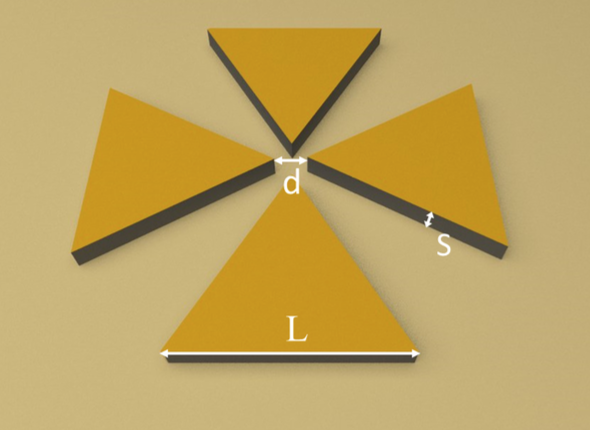
\includegraphics[trim = 0 0 0 0,  clip= true, width = 0.5\textwidth]{./pics/double_bowtie_antenna_schematic.png}}
				\caption[Schematic of a double bowtie antenna]{Schematic of a double bowtie antenna \cite{rahbany2016towards, Rahbany2015, Rahbany2016}.}
				\label{fig::double_bowtie_antenna_schematic}
		\end{figure}

		This antenna design utilizing a symmetric arrangement of four identical triangle-shaped blocks, separated by a small gap. This setup allows \LSP modes local to individual blocks to couple with each other resulting in the formation of an intense hot-spot in the center area \cite{ghenuche2008spectroscopic}, see \autoref{fig:double_bow_tie_hotspot}. The actual electromagnetic response of a double bowtie nano-antenna depends on its physical design parameters such as gap size, material used, geometry and size. Furthermore, properties of incident light such as \wl and polarization determine antenna operation.

		\begin{figure}[thp]
				\centering
				\testbox{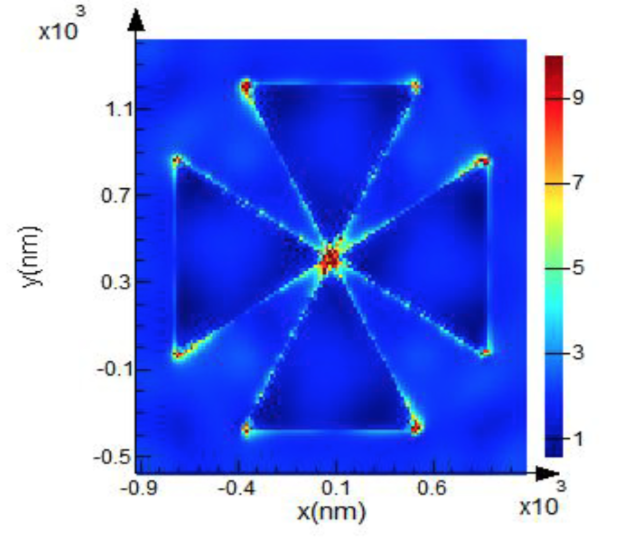
\includegraphics[trim = 0 0 0 0,  clip= true, width = 0.5\textwidth]{./pics/antenna_fdtd_simulation_field.png}}
				\label{fig::double_bow_tie_hotspot}
				\caption[Hot-spot of a double bowtie antenna]{Simulation result of the electric field map of a gold double bowtie nano-antenna \cite{rahbany2016towards, Rahbany2015, Rahbany2016}. The structure has gap of $d = \SI{150}{nm}$, a side length of $L = \SI{2}{\micro\meter}$ and a thickness of $S = \SI{60}{nm}$. The center of the antenna exhibits an area of pronounced focus, the so-called hot-spot.}
		\end{figure}


		The improved electromagnetic field at the center of a metallic nano-antenna can be used to increase the spontaneous emission rate of emitters emitting at frequencies close to the resonance frequency of the antenna. This result is the known as Purcell effect \cite{purcell1995spontaneous}. The gap between the antenna arms acts as a resonant cavity providing a strong near field interaction with the emitter. This interaction modifies the density of states of the system, effectively providing additional modes for the emitter to decay into, thus amplifying its total decay rate. The amplification affects both radiative and non-radiative decay.
		The magnitude of the amplification for an emitter is quantified by the ratio of its enhanced decay rate to its free space decay rate, known as the Purcell factor $F_p$. This factor is proportional to $Q/V_{eff}$ where $Q$ denotes the quality of the antenna and $V_{eff}$ the volume of the hot-spot. Thus antenna design must optimize $F_p$ as a necessary condition for significant enhancement of \fl emission.
		\\
		In addition to the antennas local field enhancement, the emitters original quantum yield $\eta_0$ influences the overall effectiveness of the emission enhancement. From theoretical considerations \cite{rahbany2016towards, mohammadi2008gold, mohammadi2010fluorescence, wientjes2014nanoantenna}, the modified quantum efficiency $\eta$ of the combined system consisting of emitter and antenna can be obtained as

		\begin{equation}
			\eta = \frac{\eta_0}{\frac{1-\eta_0}{F_p} + \frac{\eta_0}{\eta_{ant}} },
		\end{equation}

		where $\eta_{ant}$ denotes the fraction of \fl which is not dissipated through losses in the metal of the antenna. It is clear that an emitter with $\eta_0 \to 1$ will not profit from the Purcell effect. On the contrary, for realistic antennas with $\eta_{ant} < 1$ antenna-induced losses reduce the overall quantum yield $\eta$. Consequently poor emitters with low initial $\eta_{0}$ stand to profit the most from antenna-emitter coupling provided antennas are engineered well, \i.e.\ they maximize their Purcell Factors and minimize their losses. For an in-dept review of plasmonic nano-antennas we refer the reader to \cite{rahbany2016towards} and references therein.
		\\
		The presented considerations illustrate that due to their relatively low quantum efficiency, \sivs are excellent candidates for coupling with antennas. Thus it is promising to exploit the improved electromagnetic field at the center of a double bowtie antenna to enhance the spontaneous emission rate of \sivs and thus improve their merit as \spss.

	\subsection{Plasmonic Antenna Design and Simulation} \label{sec::structure_antenna}

		 To couple \sivs to optical antennas, we work with gold double bowtie antennas on a gold substrate. In comparison with triangular, or single bowtie antennas, double bowtie antennas offer significantly improved intensity enhancements. Antennas were provided by \nancy in a joined effort to explore the possibilities of combining antennas with \sivs. The antennas themselves were fabricated using electron beam lithography, a technique suitable to imprint predetirmined patterns onto a suitable substrate with nano-scale resolution \cite{pease1981electron}. \autoref{subfig::antenna_structures_sem} shows a SEM image of an array of antenna structures of various sizes. In \autoref{subfig::antenna_one_structure_sem} a detail of an individual double bowtie antenna is shown. It can be seen that the double bowtie antenna is placed in the center of another structure, a so-called bulls-eye antenna, consisting of multiple concentric gratings. When illuminated by a laser at a proper angle, the gratings excite surface plasmon polaritons (SPPs) which are directed towards the center of the structure. If a double bowtie antenna is present in the center, SPPs can interact with the \LSPs of the double bow tie, leading to an even stronger localization of electromagnetic fields in the gap of the bowtie. While this interaction certainly merits exploration in the context of enhancing \sivs, we omit the excitation of SSPs in our first exploration of the coupling of \sivs and antennas. Thus the presence of the gratings can be ignored for our purposes. The reader interested in the details of bulls-eye antennas and their properties is referred to \cite{rahbany2016towards}.

		 		\begin{figure}[htp]
		 			\begin{subfigure}[t]{ 0.49\linewidth}
		 				\centering
		 				\testbox{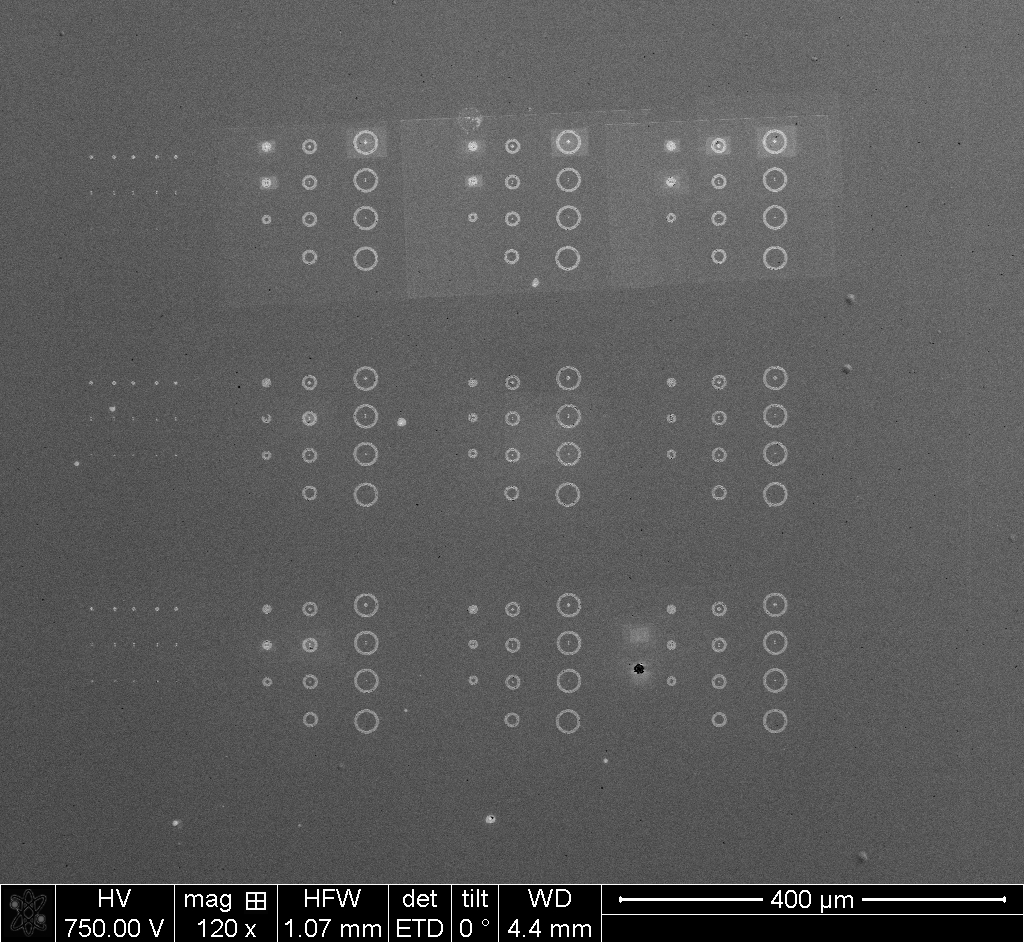
\includegraphics[trim = 0 0 0 0,  clip= true, width = 0.7\textwidth]{./pics/Antenna2_upper_right_150923_01.png}}
		 				\caption{}
		 				\label{subfig::antenna_structures_sem}
		 			\end{subfigure}
		 			\hfill
		 			\begin{subfigure}[t]{ 0.49\linewidth}
		 				\centering
		 				\testbox{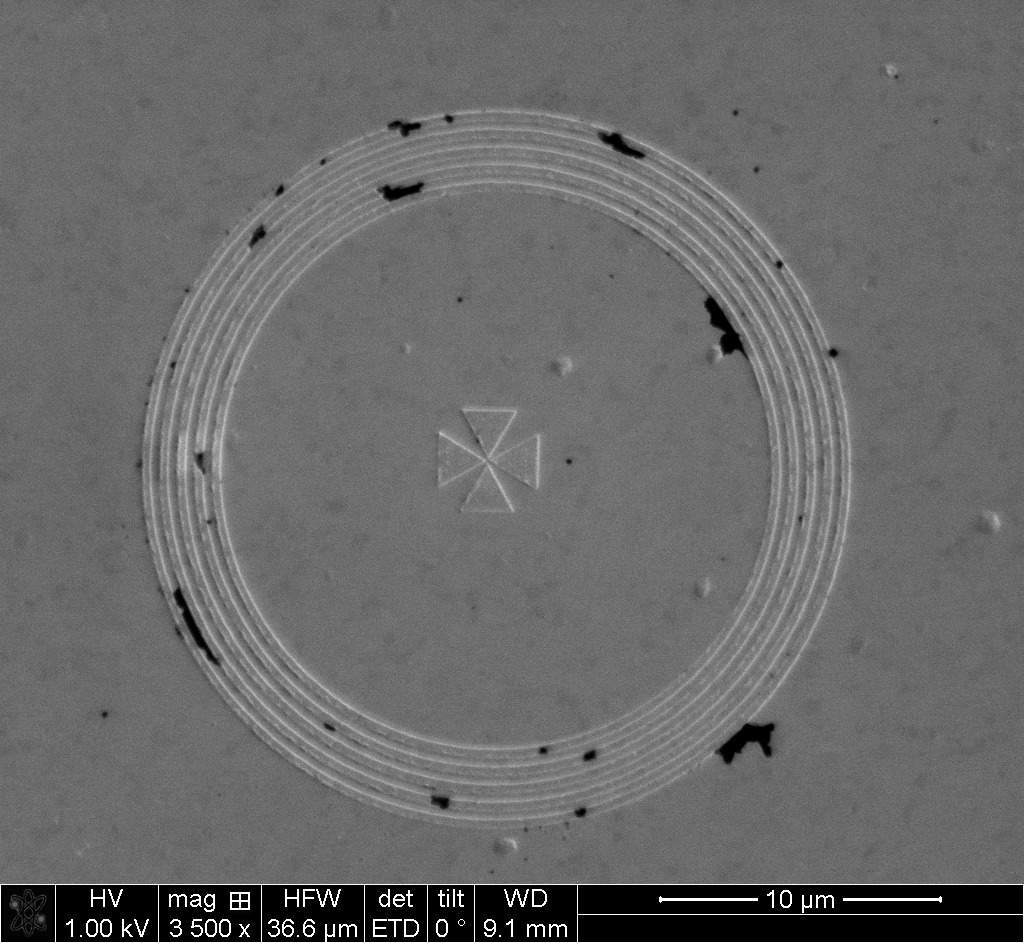
\includegraphics[trim = 0 0 0 0,  clip= true, width = 0.7\textwidth]{./pics/Ir27M_mitte_213_151111_13.jpg}}
		 				\caption{}
		 				\label{subfig::antenna_one_structure_sem}
		 			\end{subfigure}
		 			\caption[SEM images of double bowtie structures.]{SEM images of antenna structures. (a) Overview of a field of antenna structures exhibiting various dimensions. (b) Detail of one antenna sturcture. In the middle the double bowtie design is visible. A grating structure consisting of multiple gratings is surrounding it.}
		 		\end{figure}

		To effectively enhance the emission of an emitter by coupling it to an optical antenna, the emission \wl must match the resonant \wl of the antenna. In the context of \sivs a value of \SI{738}{nm} is required. Since this value can be considered constant, the design parameters of the antenna must be choose such, that the resulting resonance matches it. An additional constraint is placed on the size of the antenna gap, since it must be big enough to accommodate \nds hosting \sivs, the former are around \SI{100}{\nm} in size. However, it cannot be chosen arbitrarily big, since bigger gaps lead to larger effective volumes and thus smaller Purcell Factors.
		\\
		Using finite time difference domain (FDTD) simulation deploying Lumerical Software the design space of gold double bowtie nano-antennas on a gold substrate was explored \cite{rahbany2016towards}. Although we initially attempted to simulate antennas without a \nd present in the gap, it was subsequently discovered that its ab initio inclusion yielded superior results. Thus to determine usable design parameters for our purposes, an integrated system combining antenna and \nd was used. To better mimic experimental conditions and associated imperfections, the \nd was placed slightly off-center in the gap.
		\\
		In a series of simulation it was established that a gap-size of $d = \SI{150}{nm}$, a side length of $L = \SI{2}{\micro\meter}$ and a structure thickness of $S = \SI{60}{nm}$ are feasible parameters as referred to in \autoref{double_bowtie_antenna_schematic}. The simulation required the index of refraction for gold which was taken from Palik \cite{ghosh1998handbook}.
		\\
		The resulting geometry hosting a \nd is capable of producing a suitable hot-spot when excited.

		\begin{figure}[htp]
				\centering
				\testbox{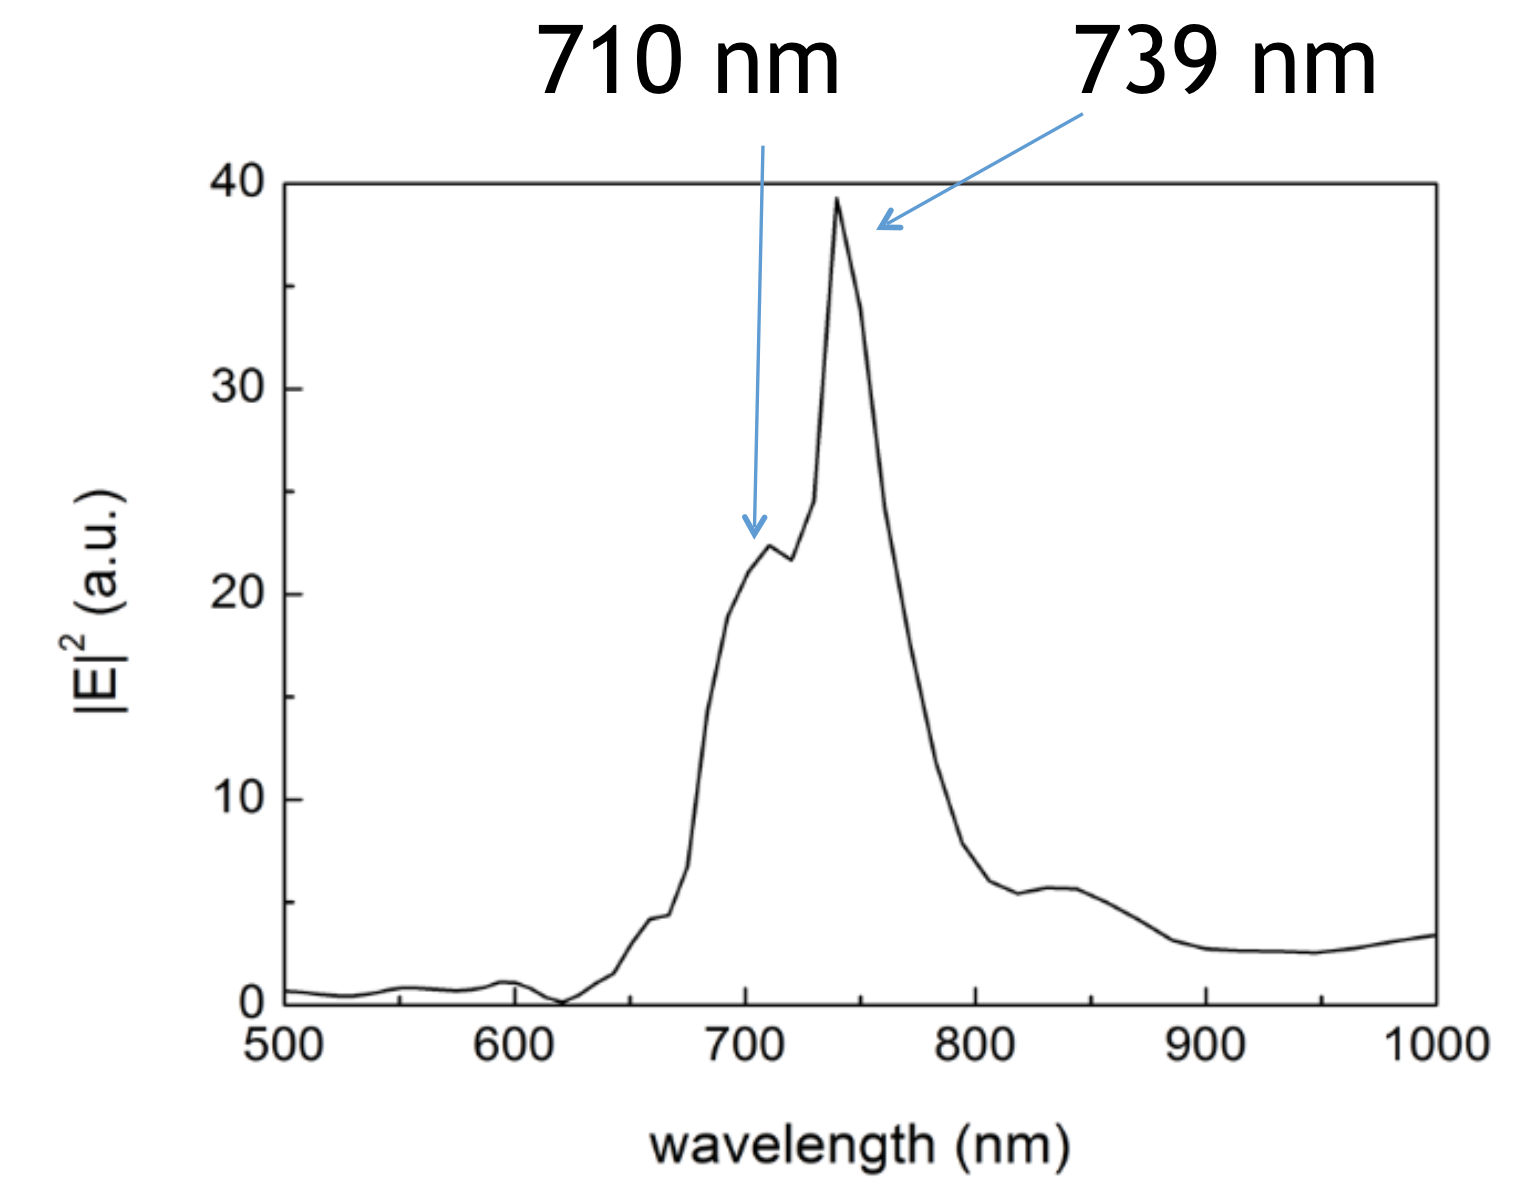
\includegraphics[trim = 0 0 0 0,  clip= true, width = 0.5\textwidth]{./pics/antenna_fdtd_simulation_spectrum.png}}
			\caption[Simulation of the resonance spectrum of a double bowtie antenna]{FDTD simulation of the electric field intensity of a double bowtie nano-antenna as as a function of the \wl of incident light. Two peaks are identified. The major peak corresponds exceptionally well with \siv emission at \SI{738}{nm}. The minor peak is attributed to the presence of a \nd.}
			\label{fig::antenna_fdtd_spectrum}
		\end{figure}

		Finally, to pin-point the resonant \wl for the antenna hosting a \nd, the electric field intensity is simulated as a function of the \wl of the incident light. The resulting spectrum is shown in \autoref{fig::antenna_fdtd_spectrum}. Two resonant peaks are found. The intense major peak at \SI{739}{nm} coincides exceptionally well with the \siv emission wavelength \SI{738}{nm} indicating successful antenna design. In addition to the major peak, an additional minor mode at a lower wavelength of \SI{710}{nm} is found \cite{Rahbany2016}. We remark that if the \nd in the gap of the antenna is removed from the simulations, the minor feature vanishes. Thus the additional peak is well-attributed to the presence of the \nd.
		\\
		In summary, the combined simulation results suggest, that the engineered system of nano-antenna and \nd is well suited to effectively enhance the emission from an \siv hosted in the \nd. In the following sections we report on the experimental realization of this preposition.

	\subsection{\siv in a Plasmonic Double Bowtie Antenna}

		In the following we report on our attempts to couple \sivs to gold double bowtie nano-antennas in order to study the properties of the resulting integrated system. Ideally, a suitable \nd containing exactly one \siv is placed in the center of the antenna. The term suitable is used to summarize both desirable spectroscopic properties such as narrow-bandwidth saturated single-photon emission as well as technical requirements such as \nd size and degree of isolation on the surface. Naturally, the odds of identifying and addressing a \nd fulfilling all these criteria simultaneously are small. 
		As a result identifying a perfect candidate for coupling is prohibitively time-consuming. 
		\autoref{fig::milky_way2} shows a $\SI{0.5}{mm}\times\SI{0.5}{mm}$ area of the surface of one of the samples which was used to identify suitable \nds.
		The black dots are \nds.
		It can be seen, that the concentration of the \nds and therefore the isolation of \nds varies.
		The black frames correspond to areas of which confocal scans were recorded to identify \nds emitting \fl.
		The red dots indicate \nds which are isolated and large enough for the \pp process and of which at least a \pl spectrum and a saturation measurement and in some cases a \gt measurement were recorded.
		Only two of the measurements performed on this sample revealed a favorable spectrum, emission saturation and at least a small dip in the \gtf indicating a small amount of \sivs.

		\begin{figure}[htbp]
			\centering
			\begin{tikzpicture}
				\begin{scope}[spy using outlines={rectangle,blue,magnification=3,size=2.5cm}]
				\node{\testbox{\includegraphics[trim = 0 0 0 0,  clip= true, width = \linewidth]{./pics/M02-16_structure2_paint.png}}};
				\spy on (-6,-4.8) in node (a) [left] at (0,-6);
				\end{scope}
			\end{tikzpicture}
			\caption[LSM scan, overview of a $\SI{0.5}{mm}\times\SI{0.5}{mm}$ area]{\Lsm scan of one of a $\SI{0.5}{mm}\times\SI{0.5}{mm}$ area of the investigated samples in search for suitable \nds. Black frames correspond to areas of which confocal scans were recorded to identify \nds emitting \fl. Red colored dots indicate \nds which are isolated enough for the \pp process and of which at least a \pl spectrum and a saturation measurement and in some cases a \gt measurement were recorded. The inset shows a magnification of the area framed in blue for better visibility of the red colored dots.}
			\label{fig::milky_way2}
		\end{figure}

		To mitigate this difficulty we decided to relax the condition of exactly one \siv per \nd and initiate our exploratory work with \nds containing several, potentially many active \sivs.
		Relying on \gt measurements we identify two interesting classes of \nds.
		The first class consists of \nds containing large ensembles of \sivs acting as coherent emitters.
		The \fl light received from large ensemble of emitters is mainly coherent, leading to a flat response in the \gtz function.
		The second class of \nds we investigate features \nds hosting multiple \sivs.
		As a result relevant \gtz measurements report weak but discernible anti-bunching dips.
		Both classes have in common that relevant \nd specimen are significantly easier to obtain than \nds containing singleton \sivs.
		Thus \nds containing ensembles of \sivs as well as \nds containing few \sivs are both valid starting points for our work.
		It is likely that the experience gained during our preliminary explorations will be valuable once \nds containing singleton \sivs become available.
		\\
		In the following sections we report on our efforts to couple \nds containing \sivs to antennas. We illustrate the coupling process and its challenges and discuss relevant results regarding the coupling of \nds of the classes described above. We close the chapter with a short discussion and suggestions for further research.

		\subsubsection{\Nds Containing Ensembles of \sivs Coupled to Antennas}\label{subsubsection::antenna_multiple_sivs}

			The \nds used for the approach of coupling ensembles of \sivs to an antenna were wet-milled from a \CVD diamond film\footnote{wet-milling performed by \muzha, diamond film grown by group of \williams}.
			The solution of \nds exhibiting a median size of \SI{100}{nm} was spin-coated on an iridium substrate treated with Piranha etch (sample of type \insituH).
			To ensure that a preselected nanodiamond exhibiting preferred optical properties can reliably be located, the iridium substrate was engraved with reference cross markers produced by a focused ion beam after the spin-coating process.
			After spin-coating, the sample was placed in an oven for \SI{3}{\hour} at \SI{450}{\celsius} to oxidize the surface and remove any residual graphite and amorphous carbon. See \autoref{ch::nanodiamonds} for more information.
			\\
			% position
			To determine the position of \nds on the original substrate, first a scan with a commercial \lsm (LSM) was performed as described in \autoref{subsec::position}.
			\autoref{subfig::cross_laser_scan} shows a part of an obtained LSM image.
			After transferring the sample into the confocal setup, confocal \fl scans of the corresponding areas are performed to identify \nds containing active emitters.
			The scanned area is shown in \autoref{subfig::pp_pl_scan}. It corresponds to the area shaded blue in \autoref{subfig::cross_laser_scan}. Thus, upon close inspection some of the bright spots appearing in the \fl scan can be associated with selected \nds in \autoref{subfig::cross_laser_scan} by eye. The correspondence between the SEM and LSM images in conjunction with the cross-markers on the substrates allows to precisely locate preselected \nds containing suitable emitter in the SEM.

			\begin{figure}[htp]
				\begin{subfigure}[t]{ 0.49\linewidth}
					\centering
					\testbox{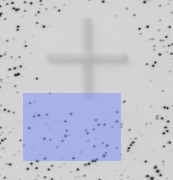
\includegraphics[trim = 0 0 0 0,  clip= true, height = 0.5\textwidth]{./pics/M05-13_structure3_stitch_crop_area.jpg}}
					\caption{}
					\label{subfig::cross_laser_scan}
				\end{subfigure}
				\hfill
				\begin{subfigure}[t]{ 0.49\linewidth}
					\centering
					\testbox{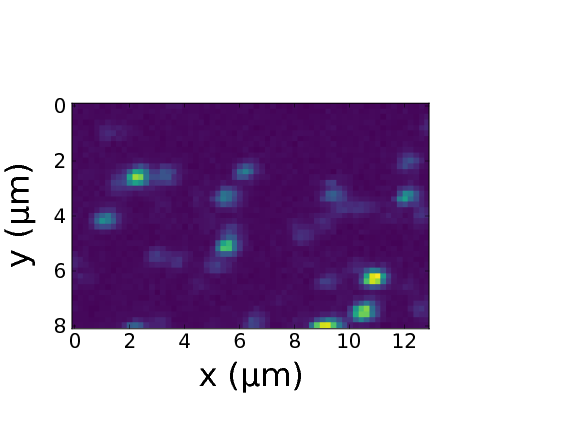
\includegraphics[trim = 0 20 70 50,  clip= true, height = 0.5\textwidth]{./pics/scan_xy-32_2APD_mum_noscale.png}}
					\caption{}
					\label{subfig::pp_pl_scan}
				\end{subfigure}
				\caption[Localizing suitable \nds]{(a) Picture recorded with a commercial high resolution laser scanning microscope. Black dots are individual \nds. The cross-marker serves as an orientation aid. The area shaded in blue represents the \pl scan in image (b). (b) \Pl scan of a
				$\SI{8}{\micro\metre} \times \SI{13}{\micro\metre}$. }
			\end{figure}

			The most promising candidate \nds are characterized by \fl spectra with very narrow \zpls and minimal \psb features. 
			\autoref{subfig::spectrum_nd_multiple} shows the spectrum stemming from one such preselected \nd.
			The \ZPL feature exhibits a \cwl of \SI[separate-uncertainty = true]{738.55\pm0.01}{nm} and a \lw of \SI[separate-uncertainty = true]{5.0\pm0.03}{nm}, corresponding well with the \ZPL of unstrained \sivs. Photon autocorrelation measurements revealed that the \nd  contains an ensemble of \sivs collectively generating coherent \fl light, see \autoref{subfig::coherent_g2}.

				\begin{figure}[htp]
					\begin{subfigure}[t]{ 0.49\linewidth}
						\centering
						\testbox{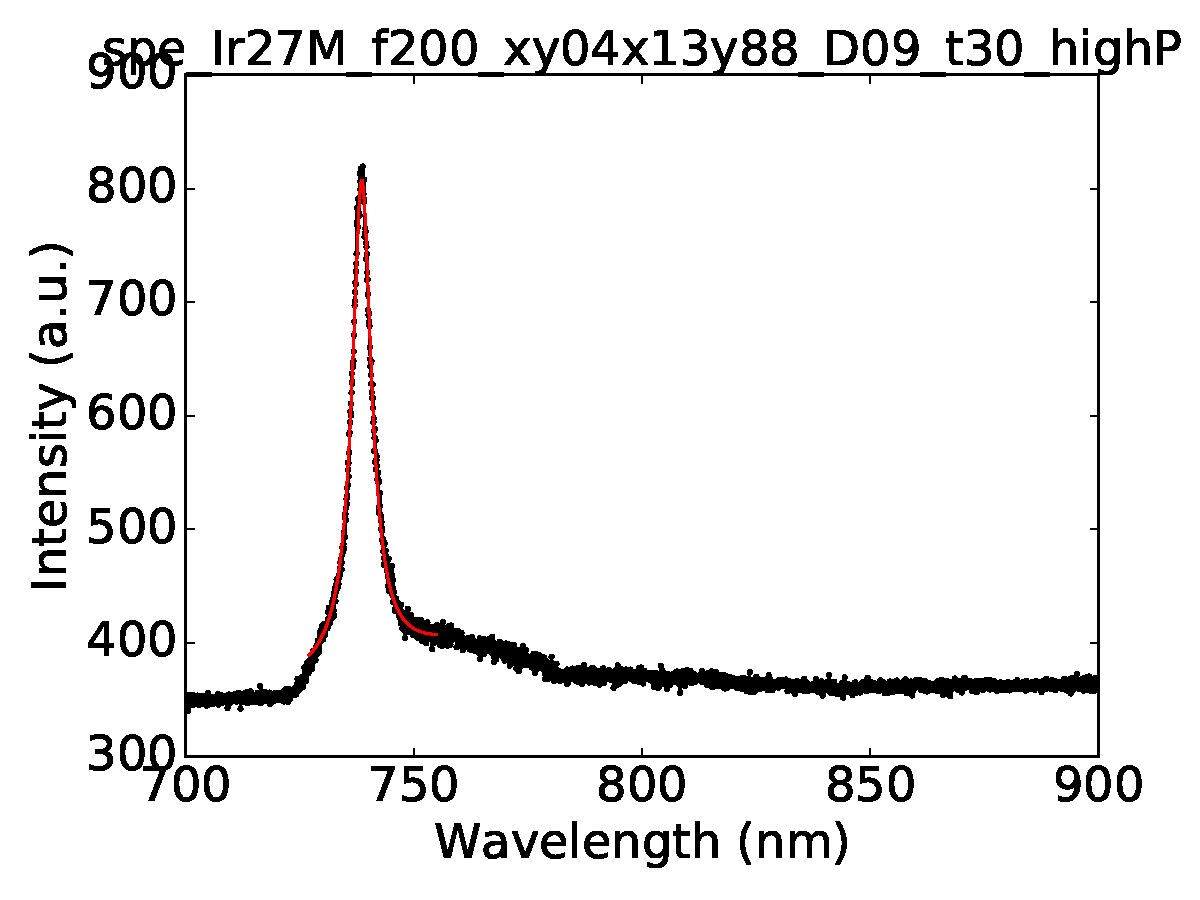
\includegraphics[trim = 0 0 0 0,  clip= true, width = 0.7\textwidth]{./pics/spe_Ir27M_f200_xy04x13y88_D09_t30_highP_fit.pdf}}
						\caption{}
						\label{subfig::spectrum_nd_multiple}
					\end{subfigure}
					\hfill
					\begin{subfigure}[t]{ 0.49\linewidth}
						\centering
						\testbox{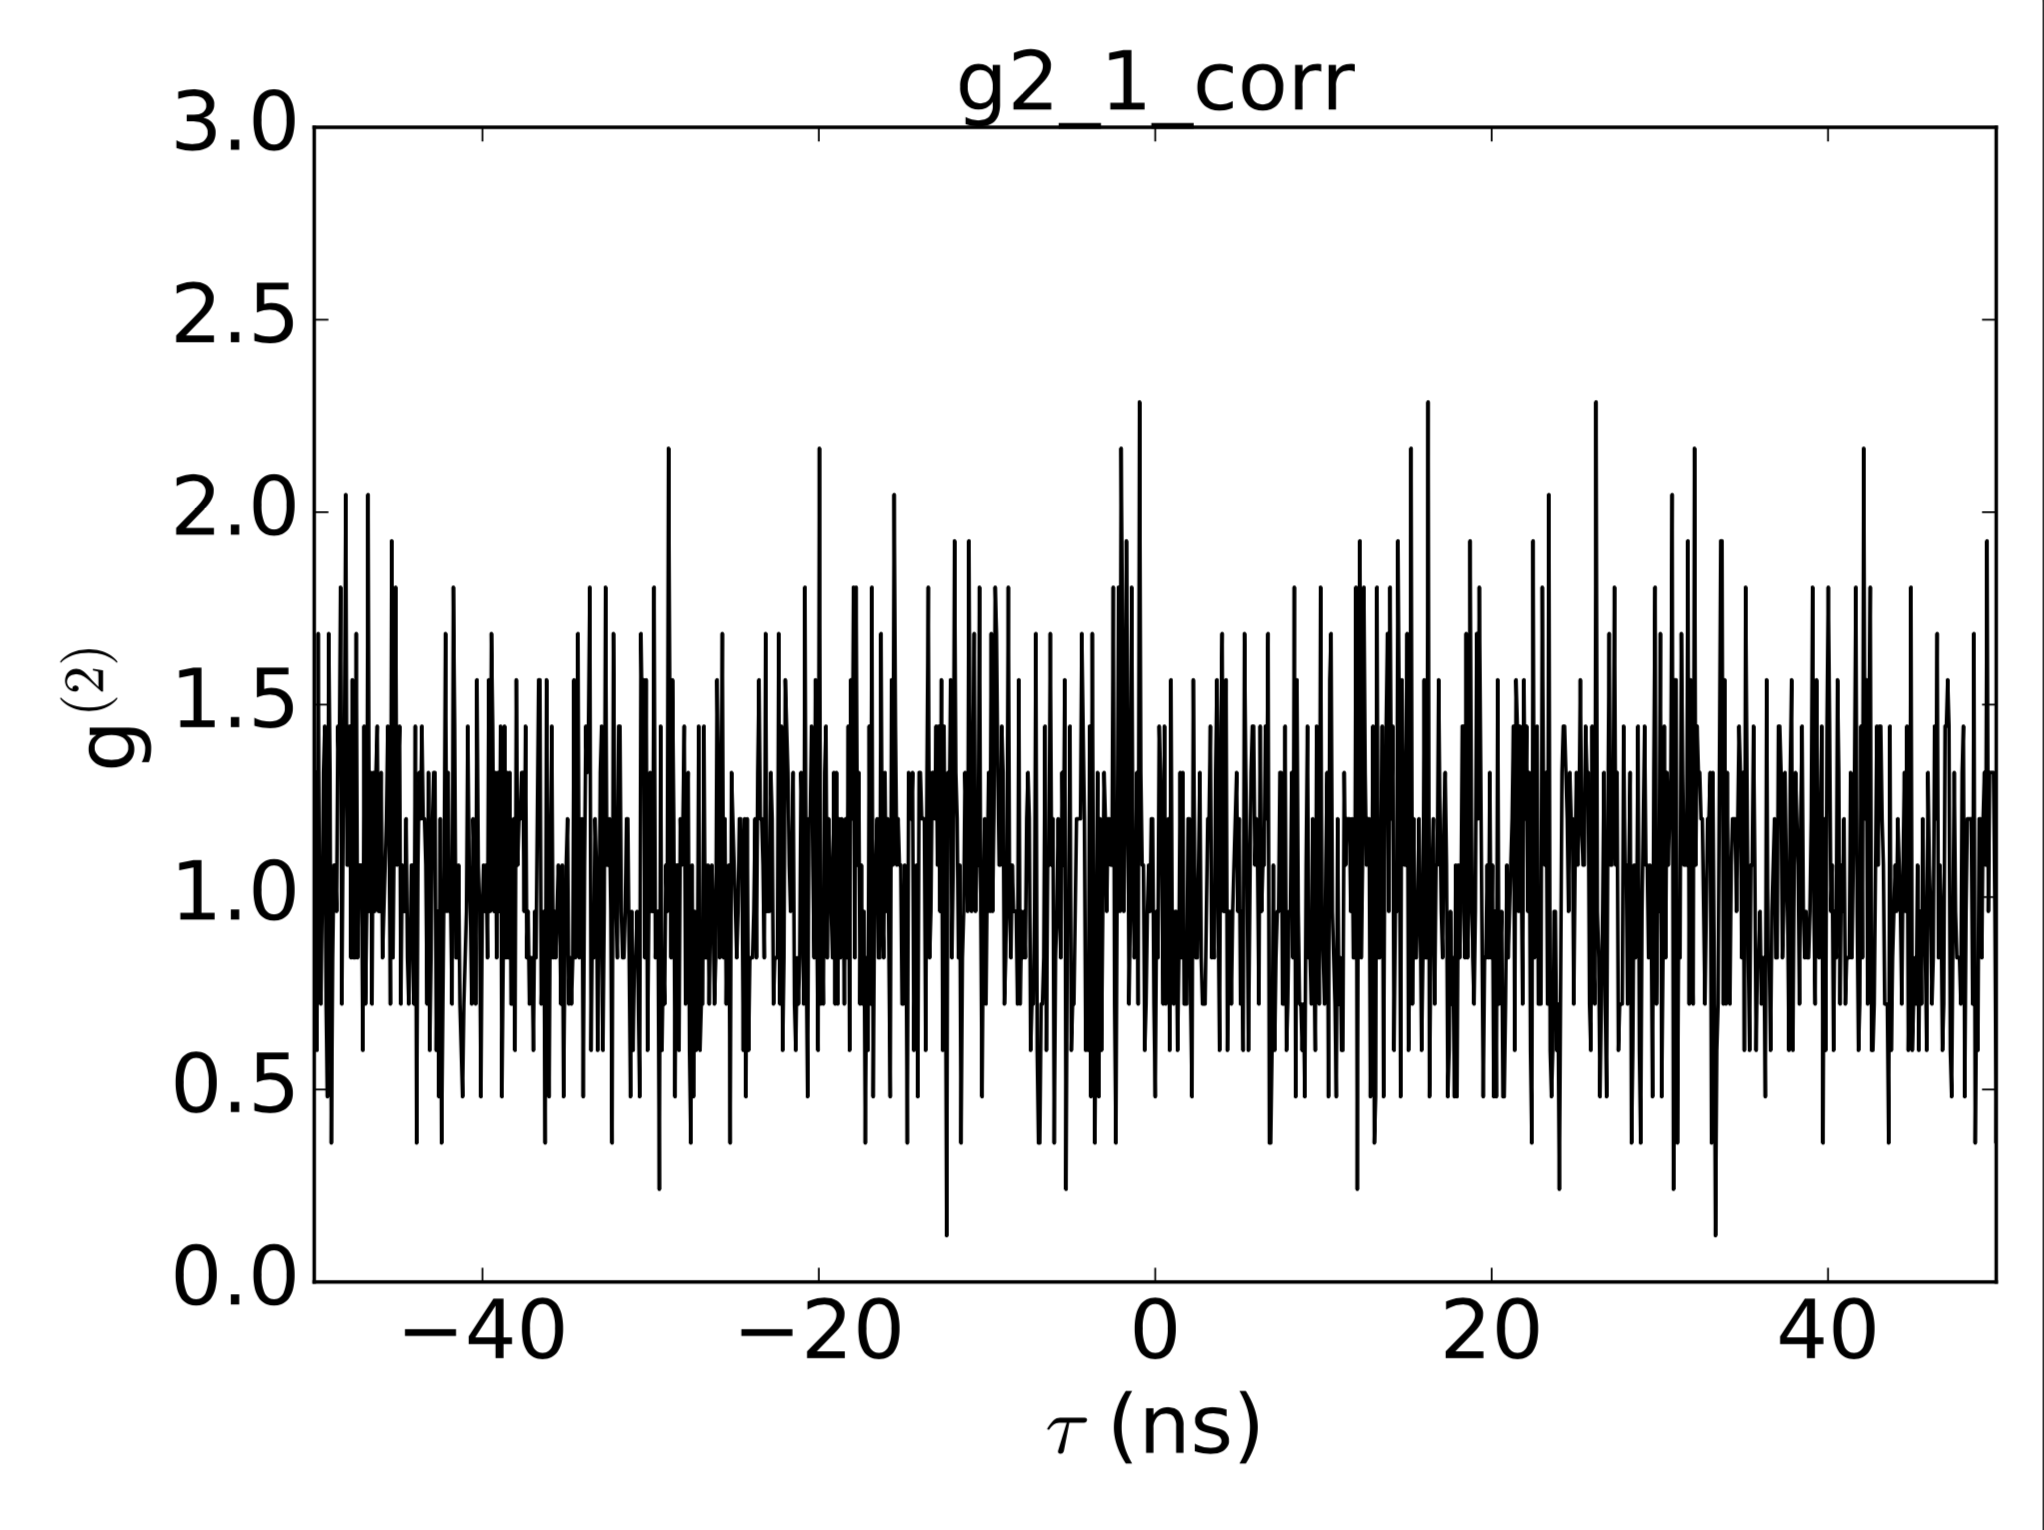
\includegraphics[trim = 0 0 0 0,  clip= true, width = 0.7\textwidth]{./pics/g2_coherent.png}}
						\caption{}
						\label{subfig::coherent_g2}
					\end{subfigure}
					\caption[Properties of a \nd containing an ensemble of \sivs]{a) PL spectrum of the emitter in the preselected nanodiamond at room temperature. Black: experimental results; red: fit to experimental data, which yields a \ZPL \cwl of \SI[separate-uncertainty = true]{738.55\pm0.01}{nm} and a \lw of \SI[separate-uncertainty = true]{5.0\pm0.03}{nm}. b) Intensity autocorrelation function recorded for the ensemble of emitters hosted by the \nd. The flat response indicates the coherent nature of the \fl light.}
				\end{figure}

			After a proper candidate for coupling with an antenna has been identified, it needs to be relocated from its original substrate to the antenna. To this end a \pp process introduced in \autoref{subsec::vcsel_structure} is used. A complete illustration of the steps involved is given in \autoref{fig::pp_antenna}.

			\begin{figure}[htp]
				\begin{subfigure}[t]{ 0.49\linewidth}
					\centering
					\testbox{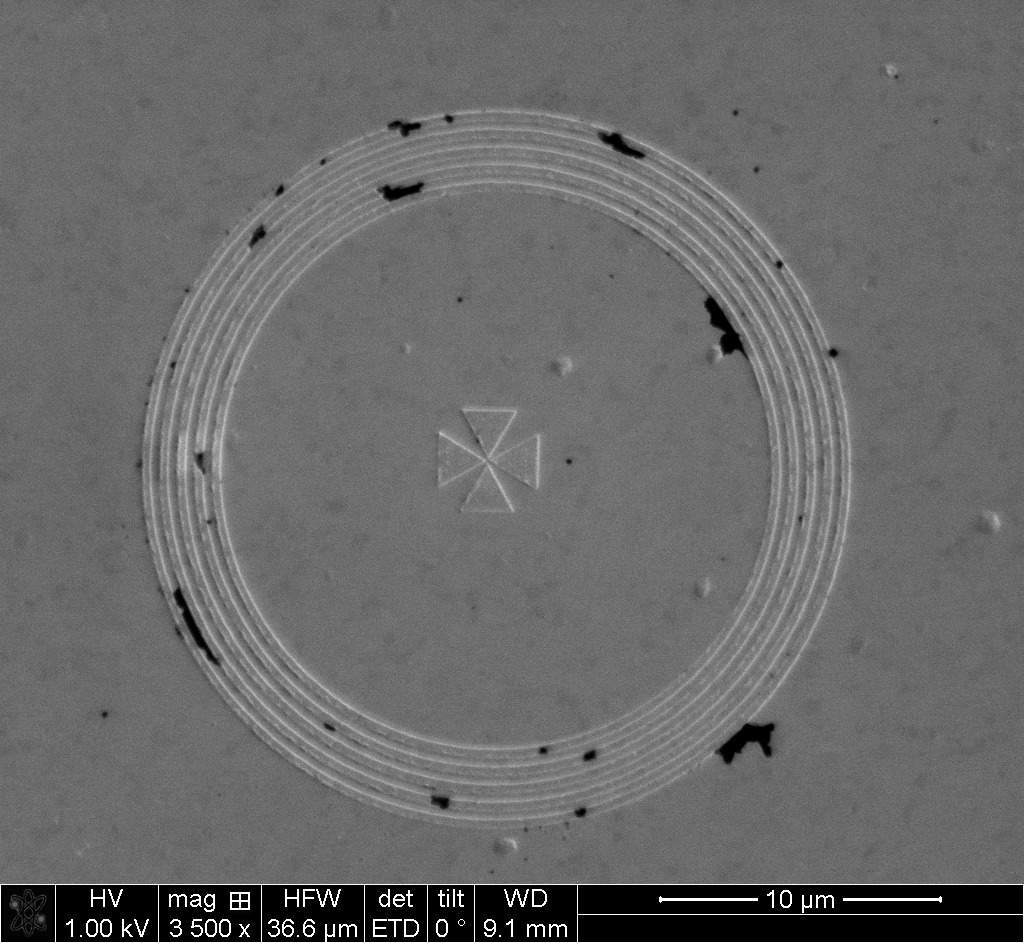
\includegraphics[trim = 0 0 0 0,  clip= true, width = 0.7\textwidth]{./pics/Ir27M_mitte_213_151111_13.jpg}}
					\caption{}
					\label{subfig::pp_target_antenna}
				\end{subfigure}
				\hfill
				\begin{subfigure}[t]{ 0.49\linewidth}
					\centering
					\testbox{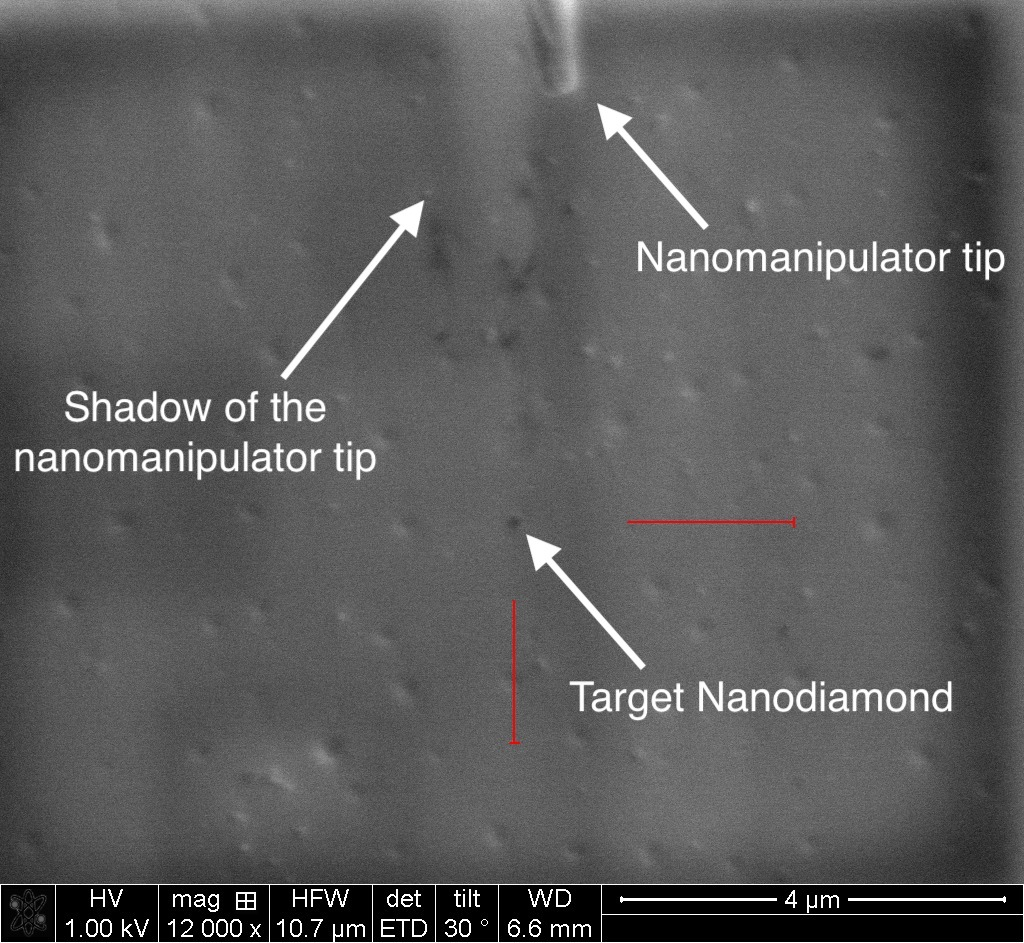
\includegraphics[trim = 0 0 0 0,  clip= true, width = 0.7\textwidth]{./pics/Ir27M_mitte_213_151111_18_edited.jpg}}
					\caption{}
					\label{subfig::pp_approach_payload}
				\end{subfigure}
				\begin{subfigure}[t]{ 0.49\linewidth}
					\centering
					\testbox{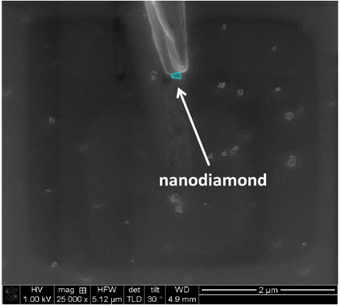
\includegraphics[trim = 0 0 0 0,  clip= true, width = 0.7\textwidth]{./pics/pick_colored.png}}
					\caption{}
					\label{subfig::pp_carry_payload}
				\end{subfigure}
				\hfill
				\begin{subfigure}[t]{ 0.49\linewidth}
					\centering
					\testbox{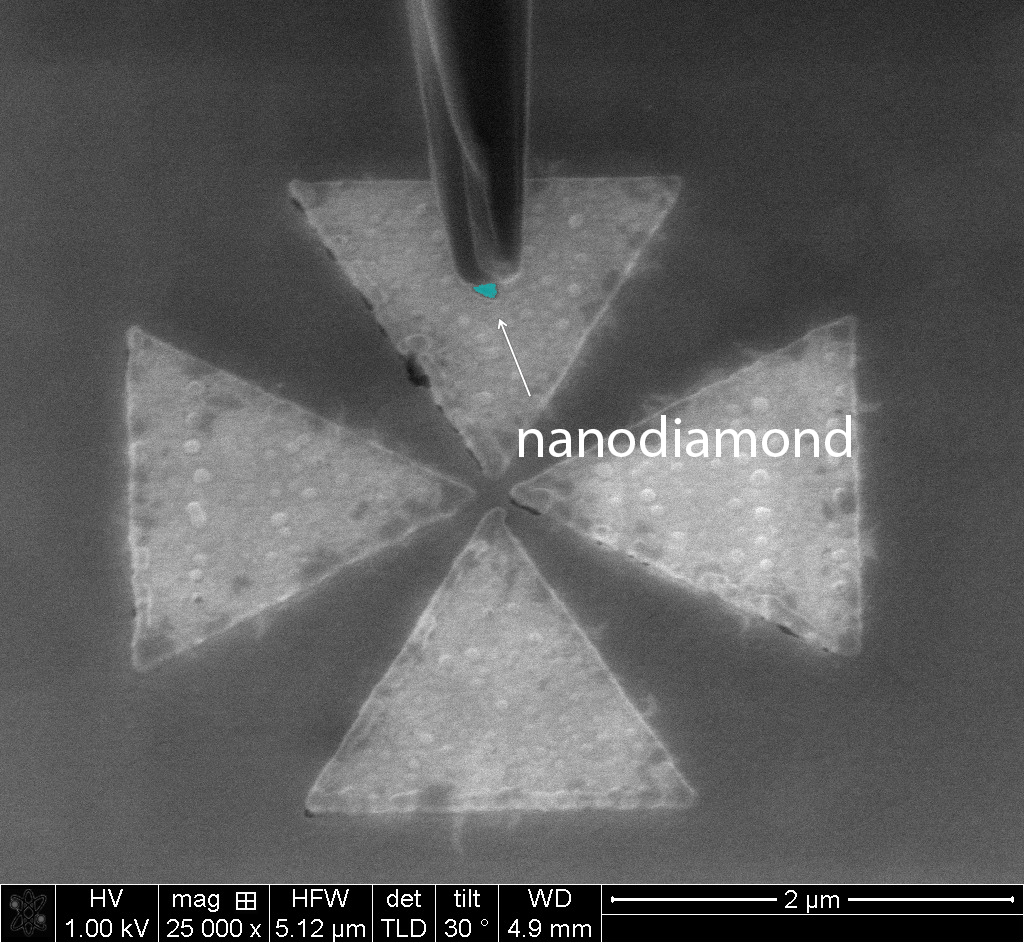
\includegraphics[trim = 0 0 0 0,  clip= true, width = 0.7\textwidth]{./pics/Ir27M_mitte_213_151111_26_colored.png}}
					\caption{}
					\label{subfig::pp_approach_target}
				\end{subfigure}
				\hfill
				\begin{subfigure}[t]{ 0.49\linewidth}
					\centering
					\testbox{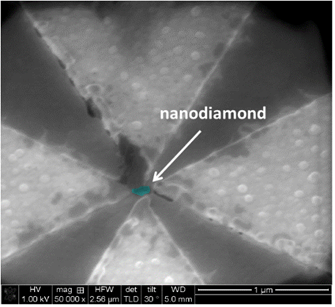
\includegraphics[trim = 0 0 0 0,  clip= true, width = 0.7\textwidth]{./pics/place_colored.png}}
					\caption{}
					\label{subfig::pp_payload_delivered}
				\end{subfigure}
				\caption[Pick-and-place coupling of \nd to antenna]{Transferring a select \nd from its original substrate to the center of a nano-antenna using \pp methods. a) Target gold double bowtie antenna on gold substrate. b) Nano-manipulator tip high-precision approaching a predetermined target \nd. c) Payload \nd sticks to the tip for transport. d) Nano-manipulator tip in high-precision approach of the antenna. e) Payload \nd was placed in the gap of the double bowtie antenna.}
				\label{fig::pp_antenna}
			\end{figure}

			The gold surface of the plasmonic antenna exhibited strong adhesion forces between the antenna surface and the \nd.
			Once the \nd touched the gold, it could not be picked up again with the tungsten tip.
			The \nd first touched the antenna structure a few nanometers away from the gap and immediately sticked to the surface, on top of one of the triangles.
			Therefore, the \nd had to be pushed into the gap with the nano-manipulator tip.
			This process caused some damage to the antenna structure.
			The damage is visible as black area at the tip of the top triangle in \autoref{subfig::pp_payload_delivered}.
			Luckily, FDTD simulations of damaged antennas reveal that this modification of the antenna hardly influences the antenna resonance.
			\\
			% Spectroscopic measurements
			After successful placement, the antenna sample is installed in the confocal setup.
			The antenna itself was located during a scan of the sample surface under white light illumination.
			A scan of the antenna is performed in the confocal setup using a \SI{660}{nm} \cw laser.
			It serves to locate the middle of the antenna structure and therefore the \nd which had been placed there.
			An outline of the rings is visible in an overview scan of the antenna structure shown in \autoref{subfig::antenna_laser_scan}.
			Zooming in to the exact center of the rings, some of the edges of the bowtie antenna are vaguely visible in \autoref{subfig::antenna_bowtie_laser_scan}.

			\begin{figure}[htp]
				\begin{subfigure}[t]{ 0.49\linewidth}
					\centering
					\testbox{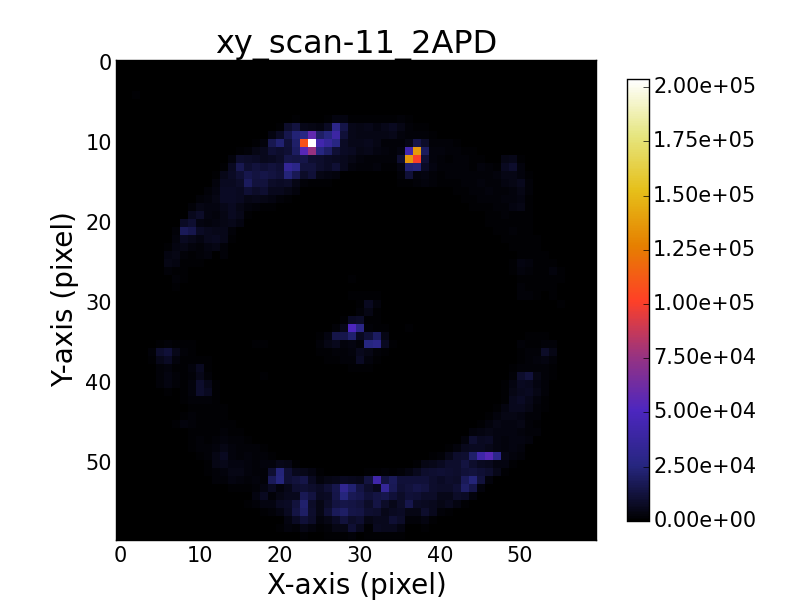
\includegraphics[trim = 0 0 0 0,  clip= true, width = 0.7\textwidth]{./pics/xy_scan-11_2APD.png}}
					\caption{}
					\label{subfig::antenna_laser_scan}
				\end{subfigure}
				\hfill
				\begin{subfigure}[t]{ 0.49\linewidth}
					\centering
					\testbox{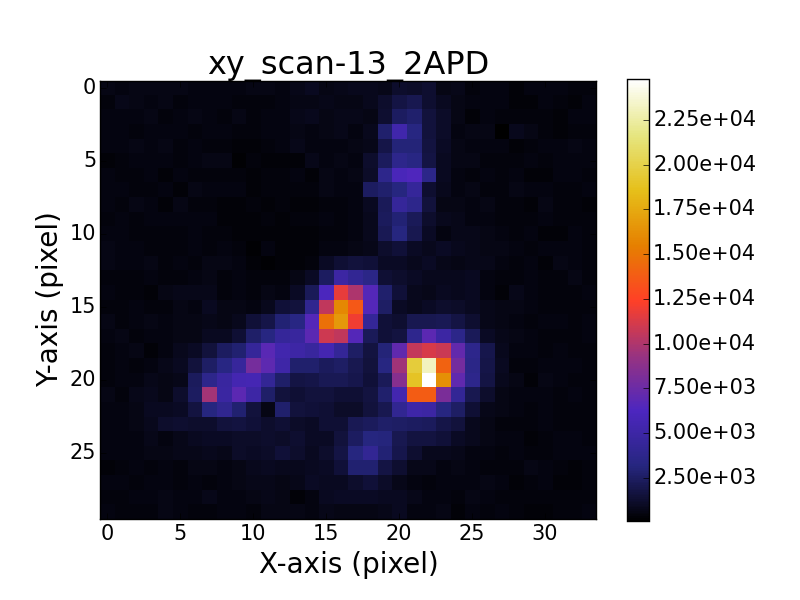
\includegraphics[trim = 0 0 0 0,  clip= true, width = 0.7\textwidth]{./pics/xy_scan-13_2APD.png}}
					\caption{}
					\label{subfig::antenna_bowtie_laser_scan}
				\end{subfigure}
				\caption[Confocal scan of a gold double bowtie antenna]{(a) Confocal scan of the double bowtie antenna where a \nd containing multiple \sivs had been placed. The rings are visible. (b) Detail scan of the triangles of the same antenna structure, which make up the double bowtie antenna. While the separate triangle cannot be seen, some edges and two bright spots are visible. To identify the place of the \nd we compare the middle point of the rings in (a), the point of intersection of the edges and the bright spot and conclude that the upper bright spot in (b) is the location of the \nd. }
			\end{figure}

			These images suffices to locate the \nd with sufficient precision to measure PL spectra.
			The PL spectrum of the ensemble of \sivs in the \nd is shown in \autoref{subfig::spectrum_antenna_nd_multiple}. It can be seen that at \SI{738}{\nm} a major peak is present, almost exactly at the same \wl than the \siv \zpl, \i.e.\ \SI{739}{\nm}. The additional minor peak at \SI{726}{\nm} is attributed to the antenna resonance mode. We remark that, any damage sustained through electron radiation during the \pp process is likely not sufficient to invalidate the \nd. This is expected as a large ensemble of \sivs can easily lose several emitters without any noticeable difference in the optical properties. Needless to say, the exact opposite is true for \nds with very few hosted \sivs making them risky to work with.
			\\
			We verified successful coupling of the ensemble of \sivs to the antenna by combining experimental and numerical results. In particular, we convolve the experimental PL spectrum of the \nd measured before placing it in the nano-antenna, see \autoref{subfig::spectrum_nd_multiple},  with the intensity spectrum of the nano-antenna obtained by means of simulations given in \autoref{fig::spectrum_antenna_nd_multiple}.
			The result of the convolution is the spectrum given in \autoref{subfig::antenna_convolution}. The agreement with the measured spectrum in \autoref{subfig::spectrum_antenna_nd_multiple} is almost perfect, indicating successful coupling of emitters and antenna. At the same time we confirm that the minor peak in \autoref{subfig::spectrum_antenna_nd_multiple} is indeed due to the antenna resonance.

			\begin{figure}[htp]
				\begin{subfigure}[t]{ 0.49\linewidth}
					\centering
					\testbox{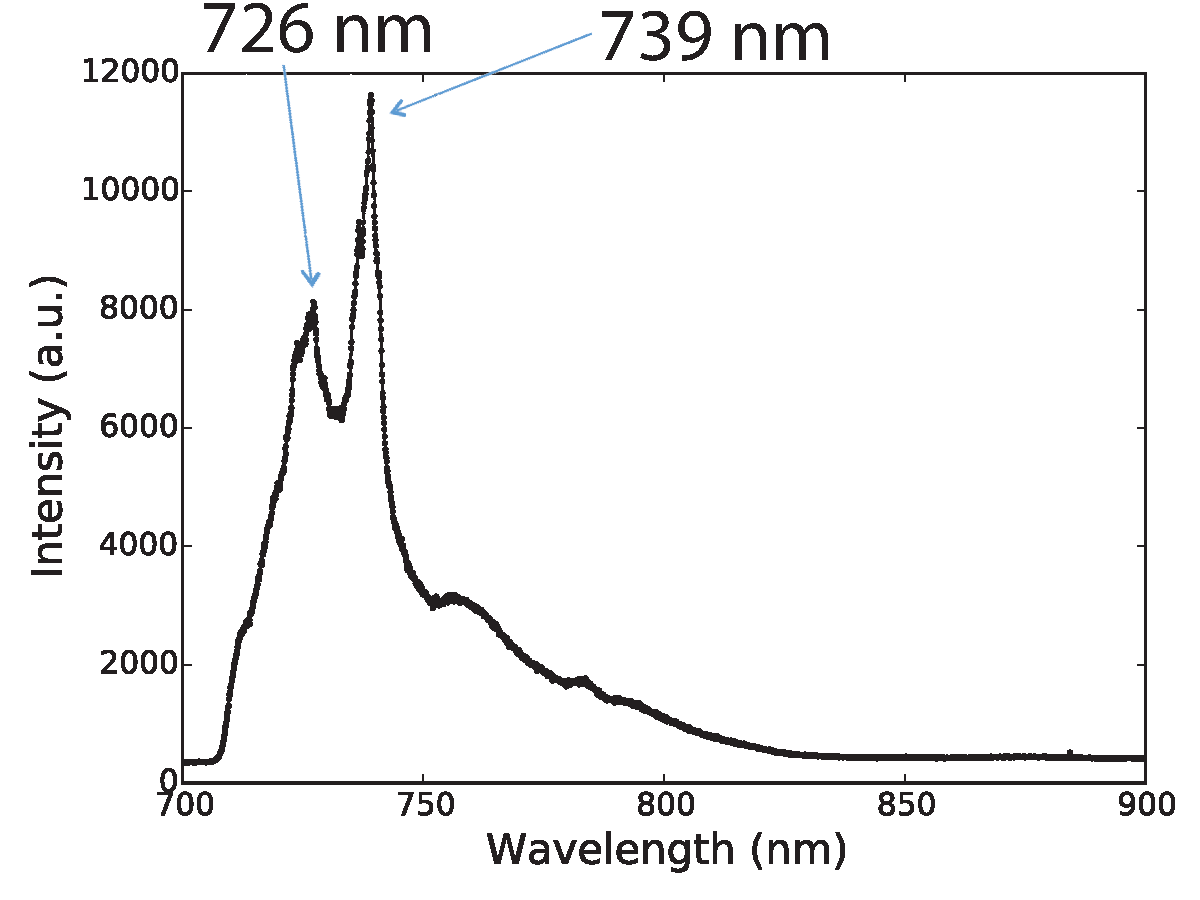
\includegraphics[trim = 0 0 0 0,  clip= true, width = 0.7\textwidth]{./pics/find_middle_with_ccd_highP_2_arrows.pdf}}
					\caption{}
					\label{subfig::spectrum_antenna_nd_multiple}
				\end{subfigure}
				\hfill
				\begin{subfigure}[t]{ 0.49\linewidth}
					\centering
					\testbox{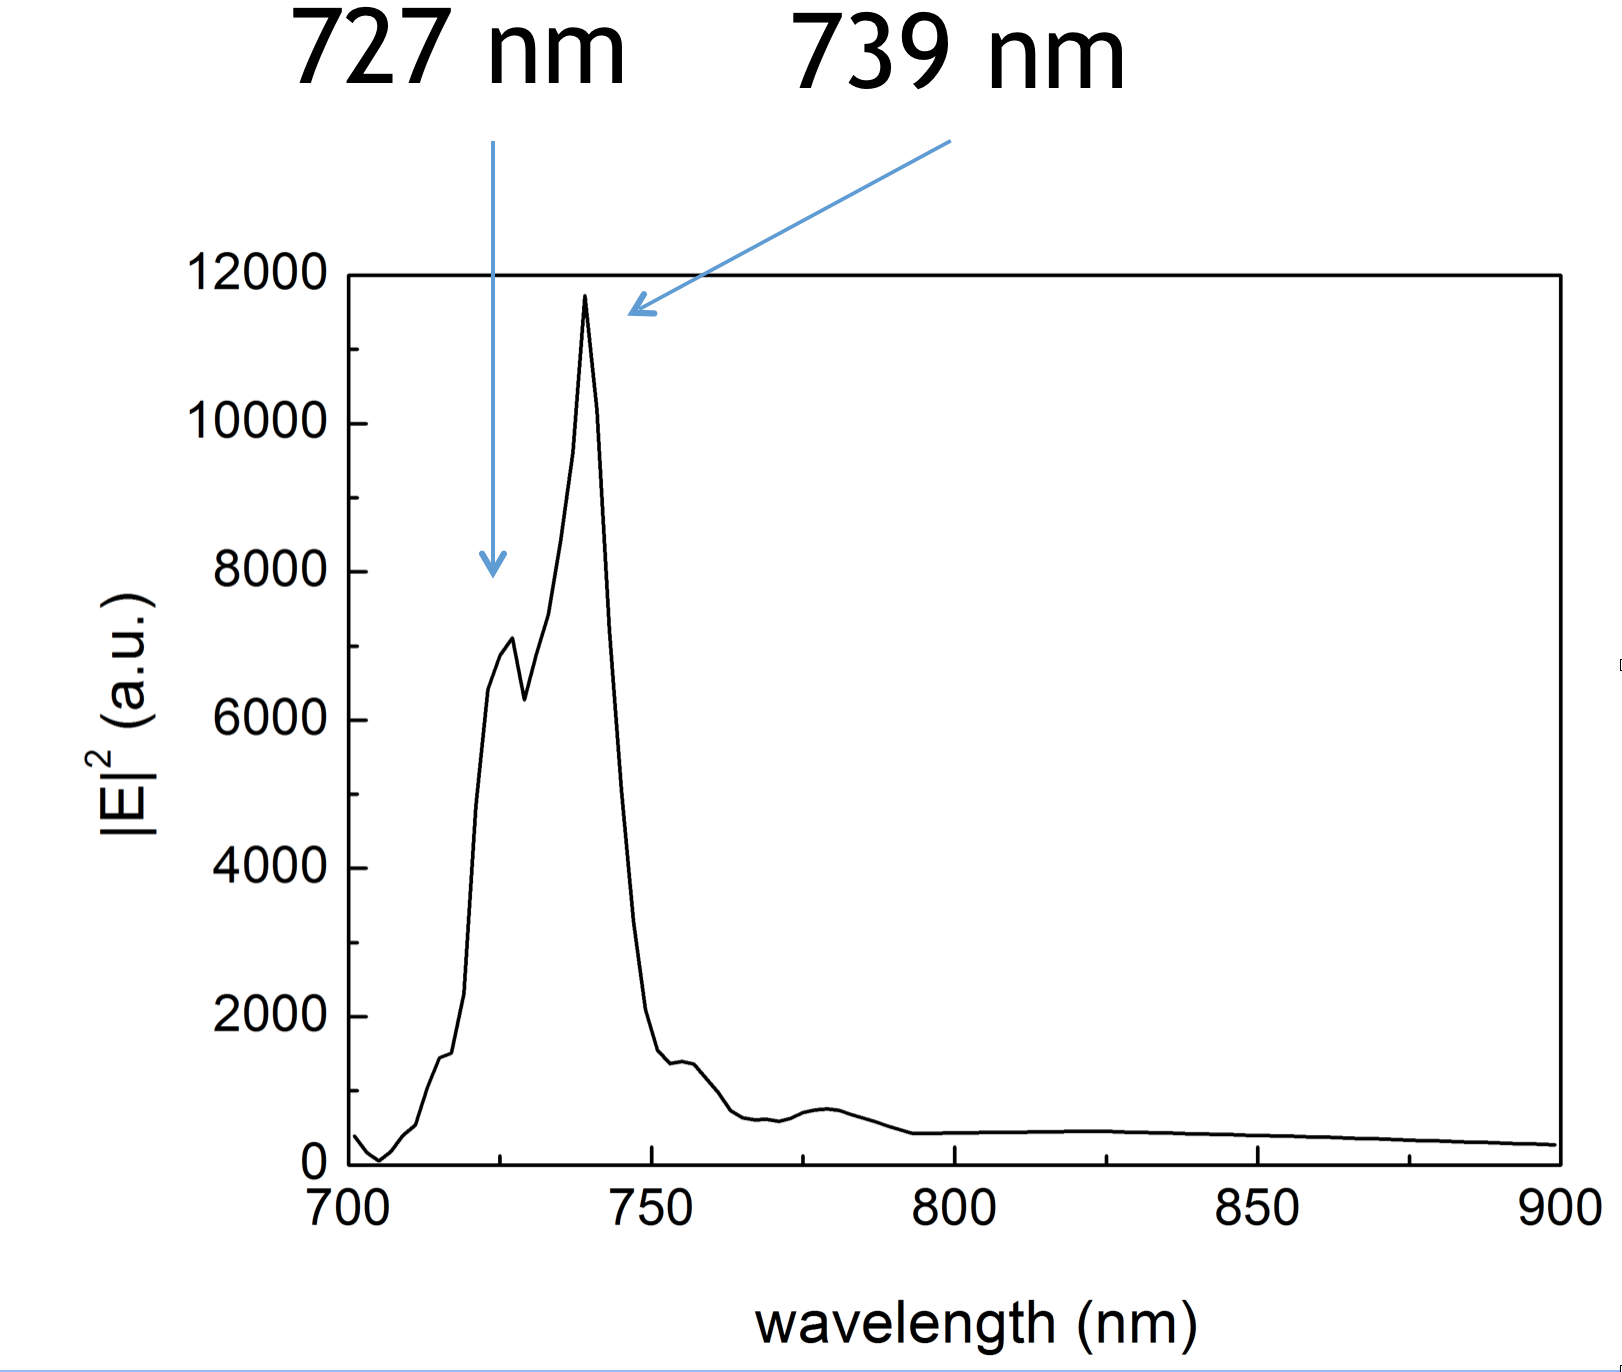
\includegraphics[trim = 0 0 0 0,  clip= true, width = 0.7\textwidth]{./pics/antenna_convolution.png}}
					\caption{}
					\label{subfig::antenna_convolution}
				\end{subfigure}
				\caption[Spectra of a \nd coupled to an antenna]{(a) Measured PL spectrum of the emitter after placing the \nd into the nano-antenna, (b) Convolution of the spectrum of the measured PL spectrum of the emitter before \pp, see \autoref{subfig::spectrum_nd_multiple}, and the simulated resonance spectrum of the nano-antenna, see \autoref{subfig::spectrum_antenna_nd_multiple}.}
			\end{figure}

			Finally, keeping experimental conditions unchanged, we measure a spectrum of an identical antenna without a \nd present in order to rule out surprising artifacts induced by the antenna itself. The resulting spectrum is given in \autoref{fig::spectrum_antenna_no_nd}.

				\begin{figure}[htp]
					\centering
					\testbox{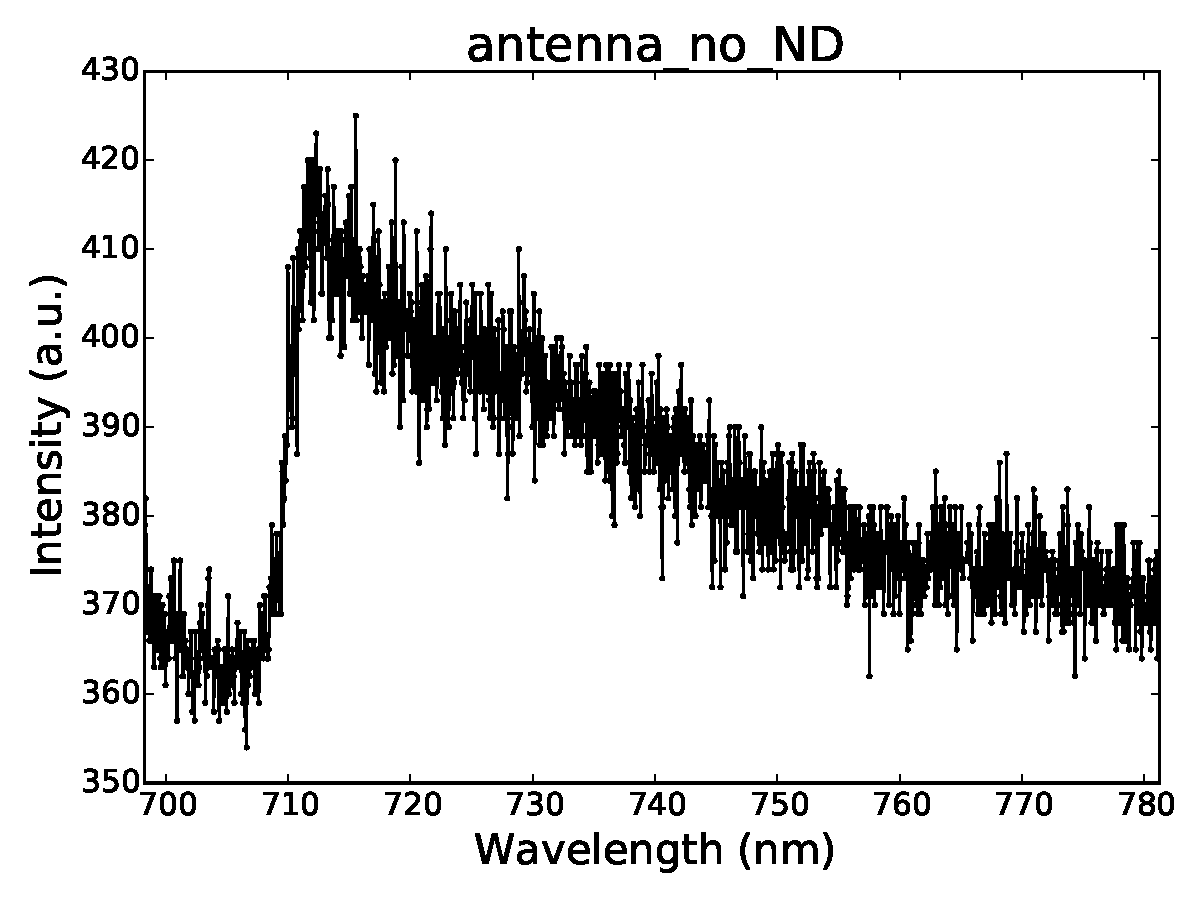
\includegraphics[trim = 0 0 0 0,  clip= true, width = 0.5\textwidth]{./pics/antenna_no_ND.pdf}}
					\caption[Spectrum of a double bowtie antenna without \nd]{Spectrum of a gold double bowtie nano-antenna without a \nd present.}
					\label{fig::spectrum_antenna_no_nd}
				\end{figure}

			At this point one must resist the temptation of comparing the values of the intensity maxima of the spectra in \autoref{subfig::spectrum_nd_multiple} and \autoref{subfig::spectrum_antenna_nd_multiple} in order to determine the enhancement the ensemble of emitters experiences. These values inherently do not allow a meaningful comparison.
			\\
			A meaningful comparison can in principle be achieved via intensity saturation measurements. By measuring the saturation intensities before and after insertion into the antenna and accounting for effects related to the polarization of emitters, the magnitude of the Purcell enhancement can be determined. Unfortunately, these methods are reserved for single emitters and do not apply for ensembles of \sivs. Thus at this point we have no method to determine the Purcell enhancement ensembles of \sivs experience.
			\\
			In summary, in this section we showed that coupling of \nds containing ensembles of \sivs with gold double bowtie antennas is feasible using a \pp approach. Furthermore we verified that the coupling is indeed present after the \nd was placed in the gap of the antenna. Unfortunately, at present there is no reliably method available to us to quantify the magnitude of \fl enhancement experienced by the \siv ensemble.

		\subsubsection{\Nds Containing Few \sivs Coupled to Antennas} \label{subsubsection::antenna_single_siv}

				\begin{remark}
					\begin{itemize}
						\item FDTD bilder fehlen komplett. Muessen unten eingefuegt werden.
						\item FDTD simulation fuer verschiedenen dipole orientations werden kurz erwaehnt, gibts da bilder?
						\item Fuer das spectrum von \nd + antenne sind die locations von den subpeaks wichtig? Irgendwo sollte erwaehnt werden, dass der neue major peak nicht dort ist wo man die \siv \zpl erwarten wuerde.
						\item Die fits an die subpeaks von dem spectrum \nd + antenne werden nicht erklaert. Wenn die nicht wichtig sind, sollte man sie zumindest beilaeufig erwaehnen.
					\end{itemize}
				\end{remark}

				After a first successful validation of inserting \nds hosting large ensembles of \sivs into a gold double bowtie antenna, we attempt to select \nds containing a comparatively small number of \sivs. Suitable \nds show an anti-bunching dip in the \gtf in addition to count-rate saturation. This can be regarded an intermediate step towards using \nds containing singleton \sivs. We stress that in comparison to \nds hosting large ensembles of emitters, \nds containing only a few emitters are already difficult to identify. Naturally, technical requirements applying to candidate \nds such as sufficiently isolation for picking it up in the \pp process and a size not larger than that of the antenna gap still need to be observed.
				\\
				% sample description
				The starting material for the \nds used here was an electronic grade diamond film produced by the company rho-BeSt coating (now renamed to CarbonCompetence).
				The film was then milled in a \basd process\footnote{\krueger} to \nds of a median size of approximately \SI{100}{nm}.
				The \nds were drop-cast at \SI{60}{\celsius} onto an \ir substrate containing cross markers. Prior to drop-casting the substrate was cleaned with Piranha etch.
				% sample M02-16: drop-casted with SiGH45
				\\
				Given samples containing \nds the tedious task of identifying potential candidates for transfer to the antenna. As described in the previous section, a commercial \lsm (LSM) is used to identify \nds on the substrate. Using the cross markers to address their exact positions, a corresponding \fl scan allow us to single out \nds with bright emission. We further test the suitability of potential candidates as follows. First, a saturation curve is recorded to establish whether the \sivs in a \nd saturate. Since saturation is a necessary albeit not sufficient condition for single-photon emission, only \nds that saturate are capable of showing an anti-bunching dip in the \gtf. Note that, measuring the \gtf potentially requires hour-long measurements, while determining saturation requires merely seconds. Thus, in search of candidate \nds we may use the saturation behavior as a quick check whether a candidate is feasible to follow on up with a lengthy \gtf measurement. For \nds containing \sivs showing saturation we then check the spectrum to assert that the emitters are indeed \sivs. After this last check \gtf measurements are established.
				\\
				After a significant search, involving a sizable number of discarded candidates, a \nd with a discernible anti-bunching dip was found. \autoref{single_siv_g2_before_transfer_antenna} shows its \gtf function while \autoref{subfig::single_siv_sat_before_transfer_antenna} reports its saturation curve. While the dip in \gtf is quite weak, it is present and a fitting it was possible. This indicates that the \nd neither contains a singleton \siv nor does it host enough \sivs to emit coherent light. Thus we conclude that a limited number of \sivs must be present. While it is not possible to quantify the number of emitters directly, the candidate sufficiently differs from \nds hosting large ensembles of \sivs. Thus it is viable to take it to the stage of coupling.

				\begin{figure}[htp]
					\begin{subfigure}[t]{ 0.49\linewidth}
						\centering
						\testbox{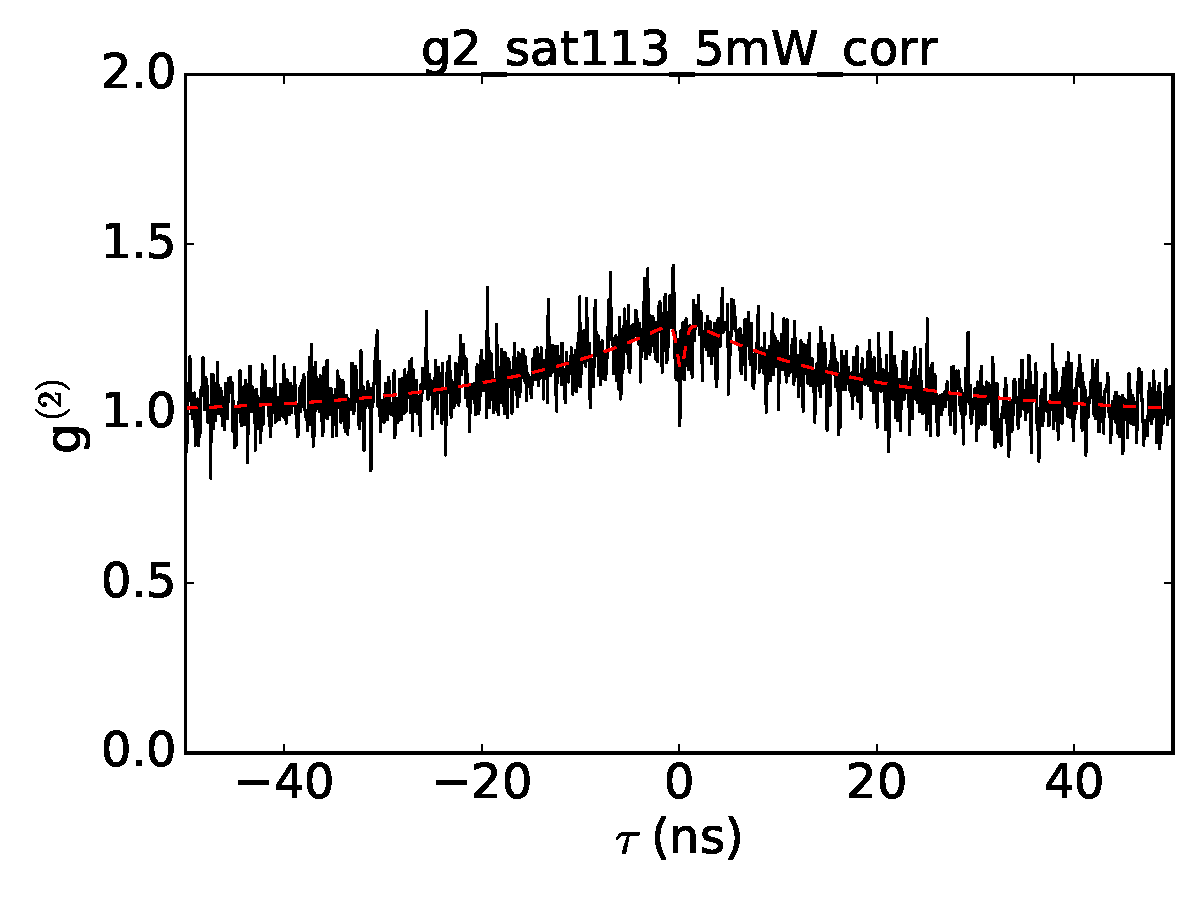
\includegraphics[trim = 0 0 0 0,  clip= true, width = 0.7\textwidth]{./pics/g2_sat113_5mW_corr_fit.pdf}}
						\caption{}
						\label{subfig::single_siv_g2_before_transfer_antenna}
					\end{subfigure}
					\hfill
					\begin{subfigure}[t]{ 0.49\linewidth}
						\centering
						\testbox{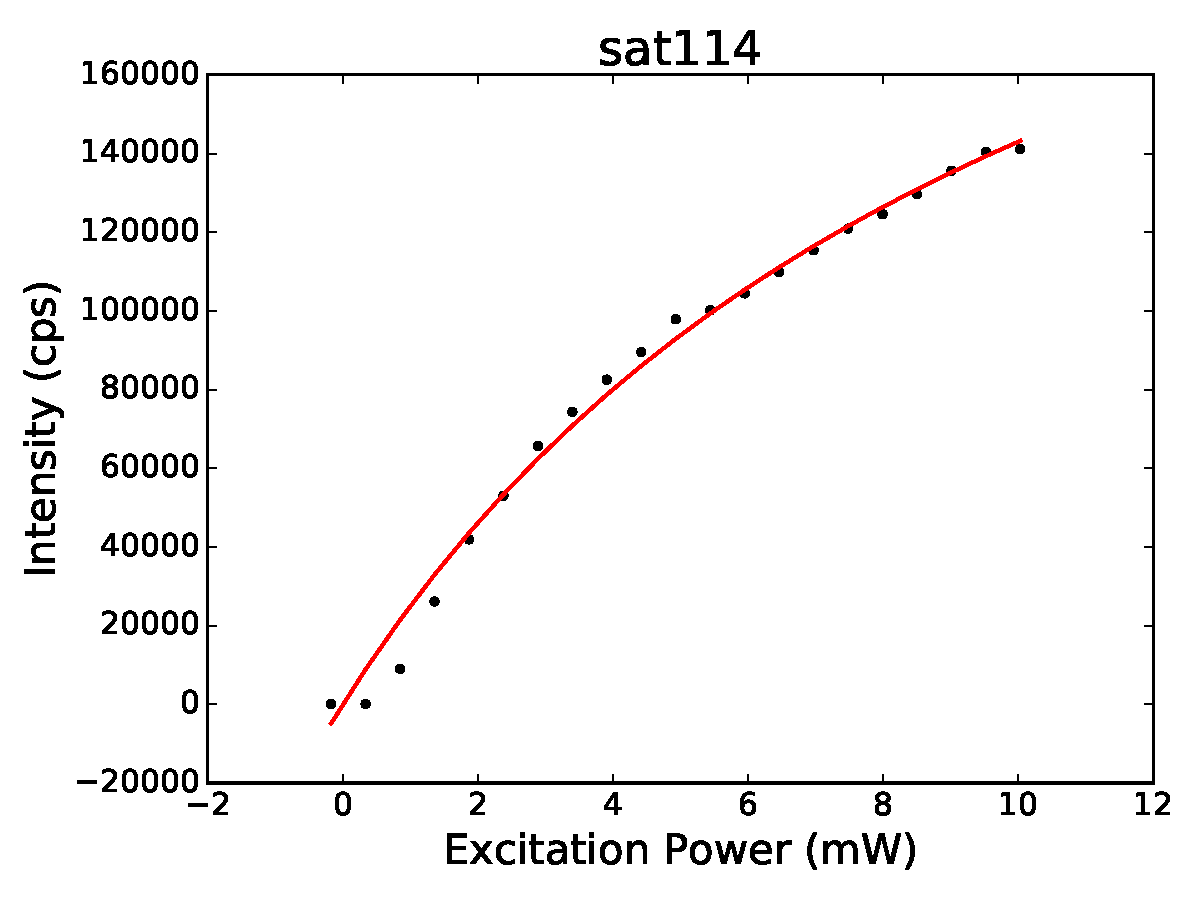
\includegraphics[trim = 0 0 0 0,  clip= true, width = 0.7\textwidth]{./pics/sat114_fit_bkg.pdf}}
						\caption{}
						\label{subfig::single_siv_sat_before_transfer_antenna}
					\end{subfigure}
					\caption[Properties of a \nd containing a few \sivs]{(a) The \gtf of the preselected \nd believed to host a limited number of \sivs. A dip at \gtz is present, however its decrease is not sufficient for a singleton \siv. This indicates that a limited number of \sivs is present since the absence of a dip can only be measured under coherent emission, i.e.\ for larger ensembles of \sivs. The dashed red line gives a fit to the data. (b) Saturation curve of the same emitter\todo[inline]{zahlen fuer sat eintragen}. Data points are black, fitted curve red.}
				\end{figure}

				In order to relocate the identified \nd to the center of a gold double bowtie antenna we repeat the \pp procedure described in the previous section, see \autoref{fig::pp_antenna}. We remark at this point that since the \nd in question contains fewer \sivs as compared to the \nds hosting large ensembles of \sivs, it is expected to be less resilient to adverse effects such as the electron radiation present during the \pp process.
				\\
				After a successful relocation, the sample containing the antenna is mounted in the confocal setup to investigate the properties of the combined system consisting of antenna and \sivs. \autoref{subfig::single_siv_spec_after_transfer_antenna} gives the spectrum of the candidate \nd after being relocated to the center of a gold double bowtie antenna. Interestingly we find a multitude of individual peaks in the vicinity of the \siv \zpl line. In addition we find that the sideband appears more pronounced in relation to the intensity of the major feature after the \nd has been relocated to the antenna. Due to the shape of the recorded sideband we conjecture that it arises as a combination of the \psbs associated with individual \sivs and additional contributions due to fluorescent contaminations. \autoref{subfig::single_siv_spec_before_transfer_antenna} showing the spectrum of the same \nd before being relocated to the antenna. Here the \psb is weaker in comparison to the \zpl feature.


				\begin{figure}[htp]
					\begin{subfigure}[t]{ 0.49\linewidth}
						\centering
						\testbox{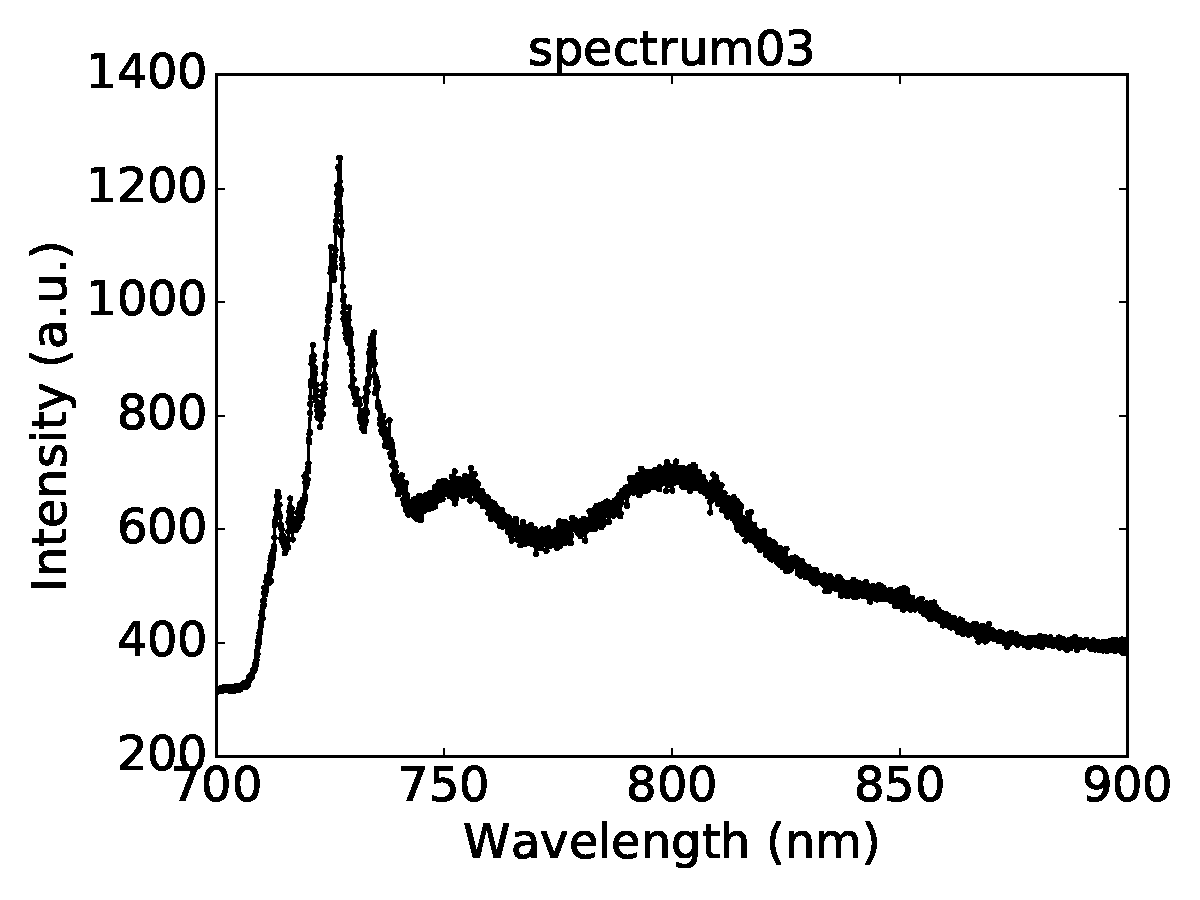
\includegraphics[trim = 0 0 0 0,  clip= true, width = 0.7\textwidth]{./pics/spectrum03.pdf}}
						\caption{}
						\label{subfig::single_siv_spec_after_transfer_antenna}
					\end{subfigure}
					\hfill
					\begin{subfigure}[t]{ 0.49\linewidth}
						\centering
						\testbox{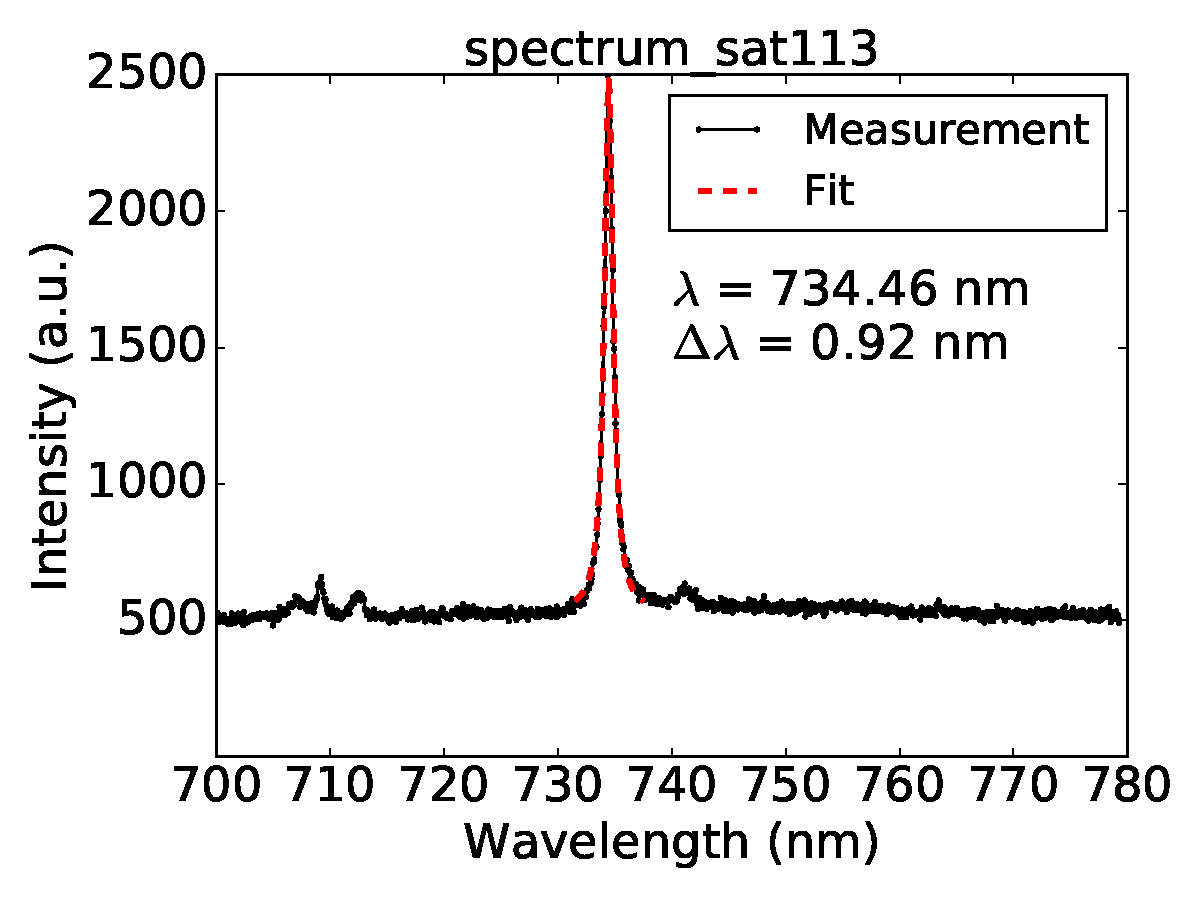
\includegraphics[trim = 0 0 0 0,  clip= true, width = 0.7\textwidth]{./pics/single_spectrum_sat113_fit.pdf}}
						\caption{}
						\label{subfig::single_siv_spec_before_transfer_antenna}
					\end{subfigure}
					\caption[Spectrum of preselected \nd containing few \sivs]{(a) Spectrum of the preselected \nd hosting few \sivs after being relocated to the center of a double bowtie antenna. (b) Spectrum of the same \nd before relocation.}
				\end{figure}

				To exclude the possibility that the obtained peaks are artifacts due to misalignment of the experimental setup, we rechecked the alignment which proved to be precise.
				\\
				To reverify the obtained spectrum, we repeated the measurement. Unfortunately, we obtained an entirely different result, showing only a broad \bkg seen in \autoref{subfig::single_siv_spec_bkg_antenna}. After checking in the confocal scan that the measurement was performed at the correct position, we had to conclude that all of the \sivs hosted by the \nd permanently bleached after recording the spectrum seen in \autoref{subfig::single_siv_spec_after_transfer_antenna}. It is likely that continued application of energy from the laser triggered this effect as earlier independent measurements established that \sivs exhibit an increased likelihood of bleaching after being exposed to electron radiation \cite{}. Thus we conclude that the exposure to electron radiation during the \pp left the \sivs in an unstable state susceptible to bleaching.

				\begin{figure}[tp]
					\begin{subfigure}[t]{ 0.49\linewidth}
						\centering
						\testbox{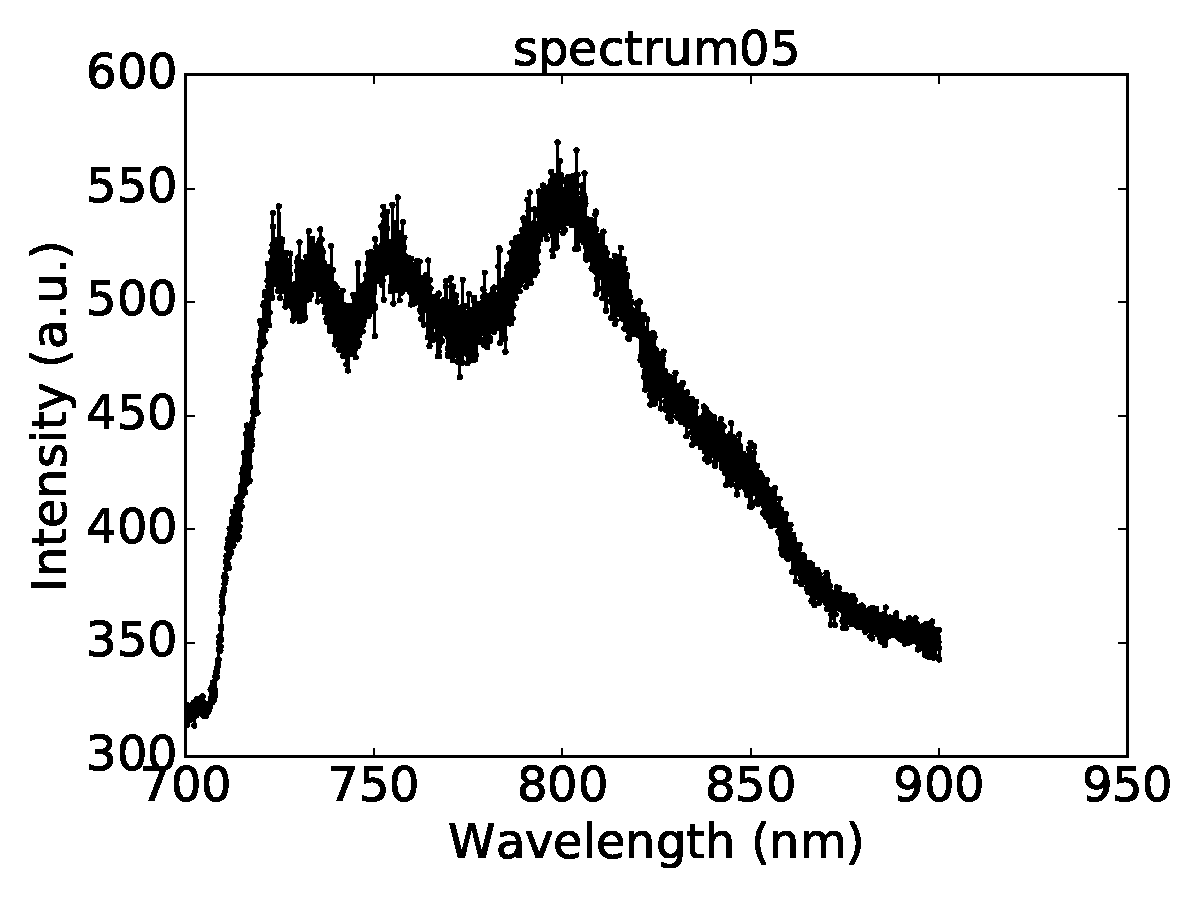
\includegraphics[trim = 0 0 0 0,  clip= true, width = 0.7\textwidth]{./pics/spectrum05.pdf}}
						\caption{}
						\label{subfig::single_siv_spec_bkg_antenna}
					\end{subfigure}
					\hfill
					\begin{subfigure}[t]{ 0.49\linewidth}
						\centering
						\testbox{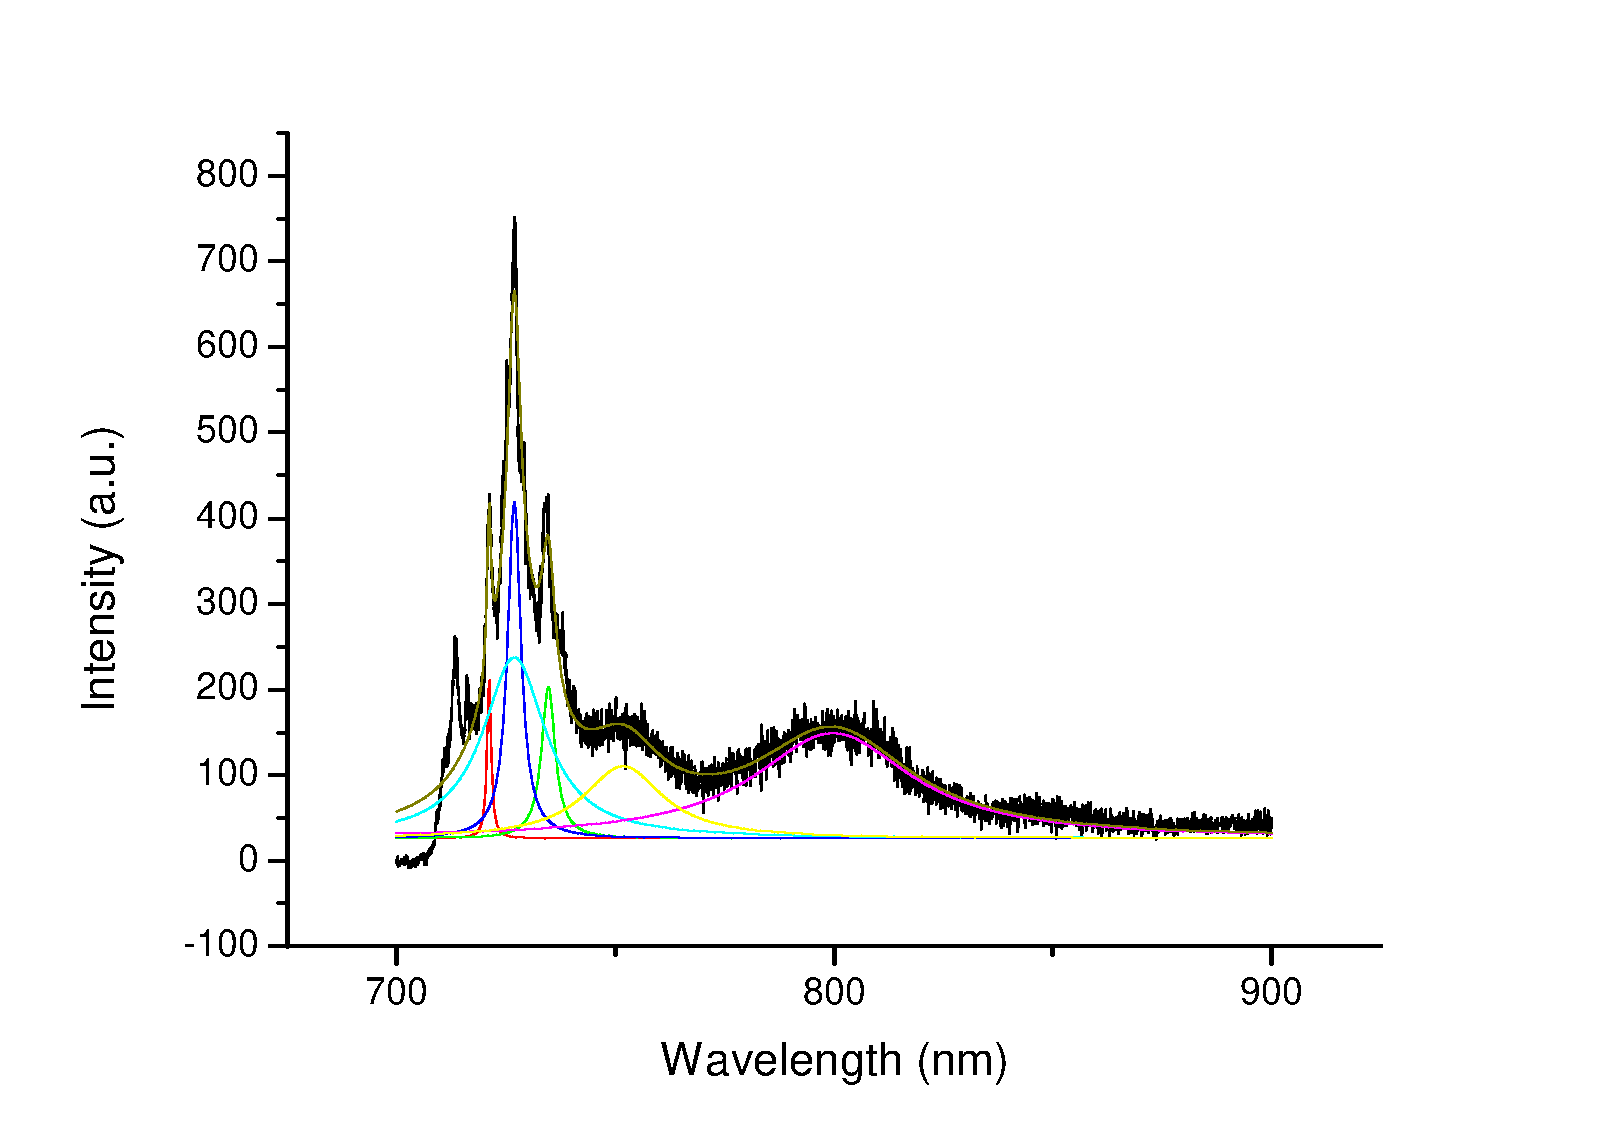
\includegraphics[trim = 0 0 0 0,  clip= true, width = 0.7\textwidth]{./pics/spectrum_sat113_fit_origin.pdf}}
						\caption{}
						\label{subfig::single_siv_spec_after_transfer_antenna_bkg_corrected}
					\end{subfigure}
					\caption[Background-corrected spectrum of a \nd in an antenna]{(a) Spectrum of the \nd hosting few \sivs coupled to the double bowtie antenna after the emitter bleached. (b) Background corrected spectrum of the transferred \nd in the double bowtie antenna. Peaks are fitted, results of the fits are the colored lines. For background correction, the spectrum in (a) was used.}
				\end{figure}

				Even though the \nd was invalidated for further measurements, the spectrum that was obtained remains to be discussed further. To better understand the obtained observations, we turn to FDTD calculations of \nd coupled to a gold plasmonic double bowtie antenna as described in the beginning of this chapter. In particular, we fold the spectrum of the \nd before insertion into the antenna as given in \autoref{subfig::single_siv_spec_before_transfer_antenna} with the simulation spectrum of the integrated system consisting of \nd and antenna. The simulation result thus constitutes a prediction of what we the spectrum in \autoref{subfig::single_siv_spec_after_transfer_antenna} should look like. \autoref{fig::fdtd_results} illustrates the simulation prediction and demonstrates that we have no reason to expect the to see the peaks between \SIrange{700}{750}{nm} observed experimentally (\autoref{fig::dipole_damaged_antenna}). Hence we must conclude that the spectrum of the \nd was modified during the \pp process. While it is not possible to pinpoint exactly which circumstance caused the modification, several effects could influence the observed spectra.
				\\
				First, the electron radiation itself. While it lacks the energy to modify the lattice itself, it can influence the electrons present and in particular may modify the charge state of \sivs. As was mentioned before, electron radiation was linked to increased likelihood of photo-bleaching.
				\\
				Next, during the \pp process it is possible that the \nd collects additional contaminating matter on its surface. Contaminations may be fluorescing themselves, thus modifying the spectrum. The fact that we record a significant sideband signal in \autoref{subfig::single_siv_spec_after_transfer_antenna} supports this conjecture.
				\\
				Yet another property of \sivs which should not be neglected is their dipole orientation interacting with the antenna. 
				% Conducting dedicated FDTD simulations with a focus on different dipole orientations indicated a dramatic effect on the resulting spectra (\autoref{fig::dipole_damaged_antenna}). 
				FDTD simulations of a damaged antenna were performed with a focus on different dipole orientations.
				While these calculations revealed a negligible effect of the antenna damage, the outcomes vary drastically for different dipole orientations (\autoref{fig::dipole_damaged_antenna}).
				We see the broad features around \SIlist{750;800}{nm} in both our experiment with few emitters (\autoref{subfig::single_siv_spec_after_transfer_antenna_bkg_corrected}) and in the simulation with dipole orientations xy and y.
				Future experiments aiming to investigate the effect of coupling \nds containing a single \siv to antennas should include polarization measurements to experimentally quantify the impact of the emitter orientation.
				\\
				% I performed some simulations on a damaged antenna with a dipole with different orientations. According to the results, I see that the antenna damage does not have a big effect on the spectra, however the dipole orientation changes the results drastically (attached picture). The results are different from what we obtained earlier with the convoluted antenna resonance method because in these simulations I am obliged to use a dipole emitter that has a broad emission and not a narrow peak at 739 nm. So I think the convolution method is much better because we start with the resonance spectrum of the antenna alone (with no emitter), and convolute that with any experimental spectrum of the emitter to predict the outcome.
				% For the new simulations, I replaced the plane wave by a dipole source that emits light with a broad emission spectrum around 739 nm. I am obliged to do that in order to have an emission spectrum of the antenna+emitter in a broad wavelength range. So yes, there is no convolution here..I just record the emission spectrum of the antenna+emitter system.
				% Even though the narrow peaks between 700 and 750 nm are not visible in the simultion, we see the broad features around 750 and 800nm in both experiment and simulation "xy" and "y"

				\begin{figure}[htbp]
					\begin{subfigure}[t]{ 0.69\linewidth}
						\centering
						\testbox{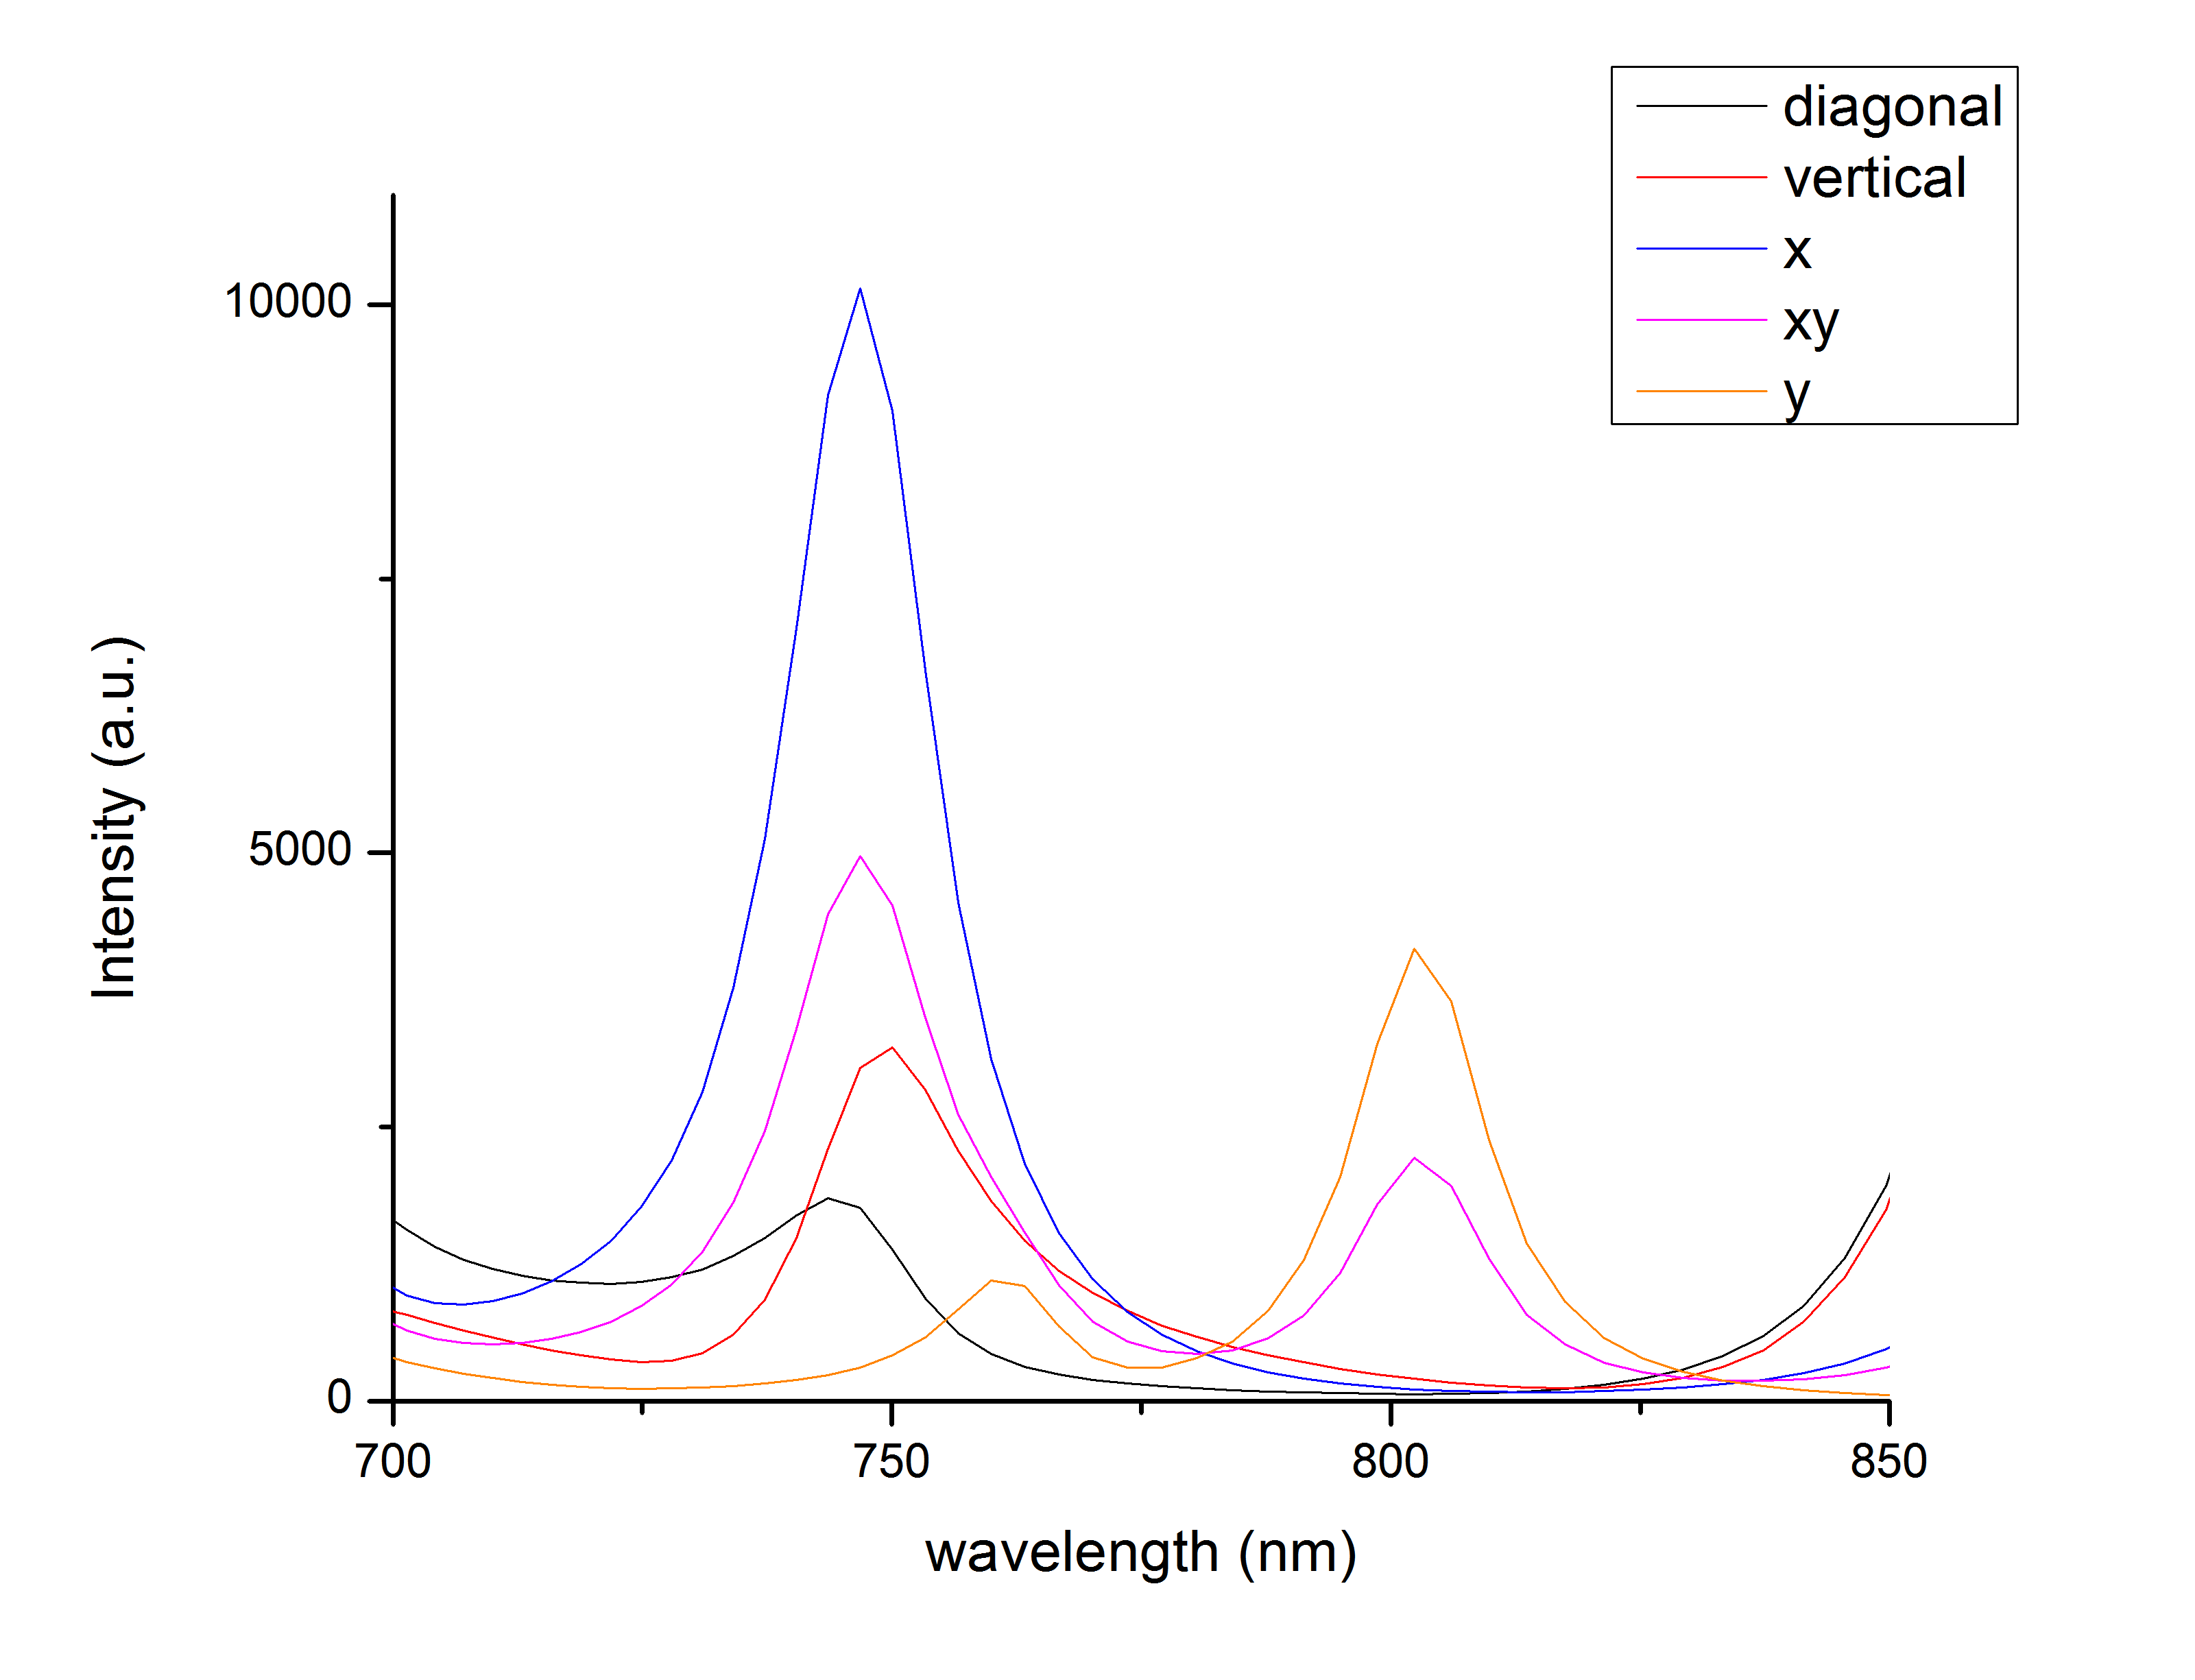
\includegraphics[trim = 0 0 0 0,  clip= true, width = \textwidth]{./pics/dipole+damaged_antenna.png}}
						\caption{}
						\label{subfig::dipole_damaged_antenna_spectrum}
					\end{subfigure}
					\hfill
					\begin{subfigure}[t]{ 0.29\linewidth}
						\centering
						\testbox{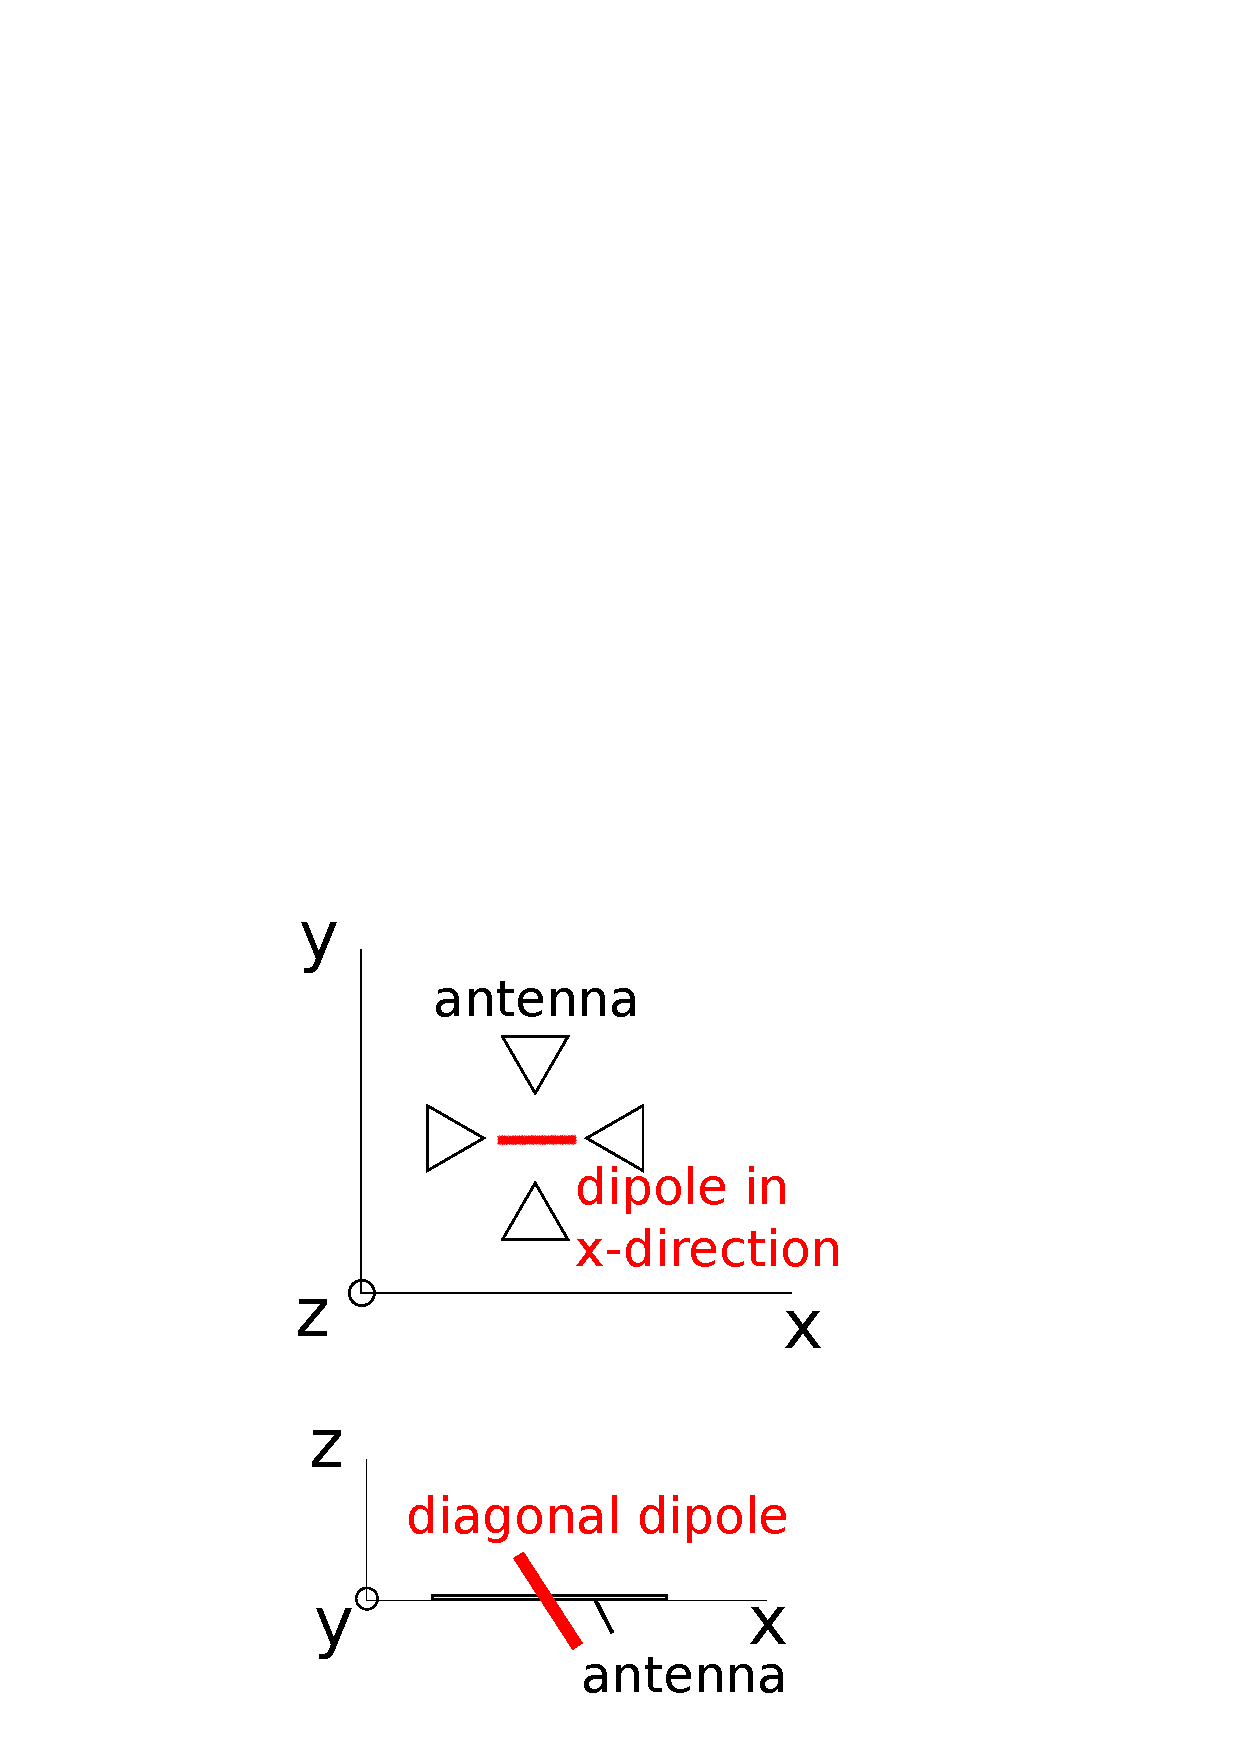
\includegraphics[trim = 0 0 0 0,  clip= true, width = \textwidth]{./pics/dipole_antenna_sketch.pdf}}
						\caption{}
						\label{subfig::dipole_damaged_antenna_sketch}
					\end{subfigure}
					\caption{(a) FDTD simulations of a dipole in a damaged antenna with different dipole orientations. Diagonal and vertical refer to out-of-plane dipole orientations, x, xy, and y are in the plane of the antenna structure. (b) Sketch visualizing the dipole orientations used in (a).}
					\label{fig::dipole_damaged_antenna}
				\end{figure}
				% To gain further insight, we performed FDTD calculations with antenna damage and different dipole orientation.
				% To be able to include the dipole orientation into the calculations, a dipole emitter with a broad emission instead of a narrow emission peak has to be used.
				% Therefore, the convolution method as described in the previsous section is more adequate for our purpose, as the \siv exhibits a very narrow emission peak.
				% However, these calculations give further insight.
				% First, the antenna damage does not have a big effect on the spectra, however the dipole orientation changes the results drastically (\autoref{}).
				As it stands, the most likely explanation of the recorded spectrum consists of a combination of the discussed effects. Since the \nd bleached almost immediately no further measurements were possible. It is thus advised to repeat the experiment hoping for a \nd that manages to complete the \pp process unharmed. At the moment it is not clear if this can be done, thus further investigation is required.

		% \subsubsection{Outlook: \Nds with single \sivs Coupled to Antennas}

		% 		To effectively quantify the emission enhancement provided by the plasmonic double bowtie antenna, a single \siv is necessary.
		% 		A correct measure for the emission enhancement is the saturation count rate since it is proportional to the inverse of the emitter's lifetime.
		% 		Hence, if there are two or more emitters present, photons of the individual emitters are emitted randomly, which renders a correct saturation measurement impossible.
		% 		However, finding \sivs in \nds which fulfill both spectroscopic (\gtz $\approx$0, saturation, narrow \ZPL spectrum) and technical (size, isolation of \nds) constraints is an extremely time-consuming process. It is a search for the needle in the haystack.
		% 		\\
		% 		We investigated different kinds of \nds in the search of \nds exhibiting optimal spectroscopic and technical parameters.
		% 		We were able to fulfill the size requirements posed by the \pp process and antenna design by producing different patches of different sizes of \nds and took the ones which were best suited.
		% 		We also developed a good isolation of the \nds on the substrate by treating the \ir substrate with Piranha etch and tuning the amount of diamond solution drop-casted onto the substrate.
		% 		This leaves us with the need of a higher probability of exactly one \siv per \nd.
		% 		Parameters which have an impact on the quantity of \sivs per \nd are the initial \siv density in the starting material and the \nd size.
		% 		Once the time constraint of finding a single \siv in a \nd is overcome, we can apply the extensive methods and knowledge gained by the reported procedures to couple a single \siv to a plasmonic bowtie antenna.
		% 		\\
		% 		To our knowledge, our experiments were the first attempts of coupling \sivs to plasmonic bowtie antennas.
		% 		The extraordinarily precise correlation of the theoretically predicted and the experimentally recorded spectrum of an ensemble of \sivs in a \nd make this process a promising candidate for future applications.
